% Options for packages loaded elsewhere
\PassOptionsToPackage{unicode}{hyperref}
\PassOptionsToPackage{hyphens}{url}
%
\documentclass[
]{book}
\usepackage{lmodern}
\usepackage{amsmath}
\usepackage{ifxetex,ifluatex}
\ifnum 0\ifxetex 1\fi\ifluatex 1\fi=0 % if pdftex
  \usepackage[T1]{fontenc}
  \usepackage[utf8]{inputenc}
  \usepackage{textcomp} % provide euro and other symbols
  \usepackage{amssymb}
\else % if luatex or xetex
  \usepackage{unicode-math}
  \defaultfontfeatures{Scale=MatchLowercase}
  \defaultfontfeatures[\rmfamily]{Ligatures=TeX,Scale=1}
\fi
% Use upquote if available, for straight quotes in verbatim environments
\IfFileExists{upquote.sty}{\usepackage{upquote}}{}
\IfFileExists{microtype.sty}{% use microtype if available
  \usepackage[]{microtype}
  \UseMicrotypeSet[protrusion]{basicmath} % disable protrusion for tt fonts
}{}
\makeatletter
\@ifundefined{KOMAClassName}{% if non-KOMA class
  \IfFileExists{parskip.sty}{%
    \usepackage{parskip}
  }{% else
    \setlength{\parindent}{0pt}
    \setlength{\parskip}{6pt plus 2pt minus 1pt}}
}{% if KOMA class
  \KOMAoptions{parskip=half}}
\makeatother
\usepackage{xcolor}
\IfFileExists{xurl.sty}{\usepackage{xurl}}{} % add URL line breaks if available
\IfFileExists{bookmark.sty}{\usepackage{bookmark}}{\usepackage{hyperref}}
\hypersetup{
  pdftitle={exposomeShiny User's Guide},
  pdfauthor={Escribà Montagut, Xavier; González, Juan R.},
  hidelinks,
  pdfcreator={LaTeX via pandoc}}
\urlstyle{same} % disable monospaced font for URLs
\usepackage{color}
\usepackage{fancyvrb}
\newcommand{\VerbBar}{|}
\newcommand{\VERB}{\Verb[commandchars=\\\{\}]}
\DefineVerbatimEnvironment{Highlighting}{Verbatim}{commandchars=\\\{\}}
% Add ',fontsize=\small' for more characters per line
\usepackage{framed}
\definecolor{shadecolor}{RGB}{248,248,248}
\newenvironment{Shaded}{\begin{snugshade}}{\end{snugshade}}
\newcommand{\AlertTok}[1]{\textcolor[rgb]{0.94,0.16,0.16}{#1}}
\newcommand{\AnnotationTok}[1]{\textcolor[rgb]{0.56,0.35,0.01}{\textbf{\textit{#1}}}}
\newcommand{\AttributeTok}[1]{\textcolor[rgb]{0.77,0.63,0.00}{#1}}
\newcommand{\BaseNTok}[1]{\textcolor[rgb]{0.00,0.00,0.81}{#1}}
\newcommand{\BuiltInTok}[1]{#1}
\newcommand{\CharTok}[1]{\textcolor[rgb]{0.31,0.60,0.02}{#1}}
\newcommand{\CommentTok}[1]{\textcolor[rgb]{0.56,0.35,0.01}{\textit{#1}}}
\newcommand{\CommentVarTok}[1]{\textcolor[rgb]{0.56,0.35,0.01}{\textbf{\textit{#1}}}}
\newcommand{\ConstantTok}[1]{\textcolor[rgb]{0.00,0.00,0.00}{#1}}
\newcommand{\ControlFlowTok}[1]{\textcolor[rgb]{0.13,0.29,0.53}{\textbf{#1}}}
\newcommand{\DataTypeTok}[1]{\textcolor[rgb]{0.13,0.29,0.53}{#1}}
\newcommand{\DecValTok}[1]{\textcolor[rgb]{0.00,0.00,0.81}{#1}}
\newcommand{\DocumentationTok}[1]{\textcolor[rgb]{0.56,0.35,0.01}{\textbf{\textit{#1}}}}
\newcommand{\ErrorTok}[1]{\textcolor[rgb]{0.64,0.00,0.00}{\textbf{#1}}}
\newcommand{\ExtensionTok}[1]{#1}
\newcommand{\FloatTok}[1]{\textcolor[rgb]{0.00,0.00,0.81}{#1}}
\newcommand{\FunctionTok}[1]{\textcolor[rgb]{0.00,0.00,0.00}{#1}}
\newcommand{\ImportTok}[1]{#1}
\newcommand{\InformationTok}[1]{\textcolor[rgb]{0.56,0.35,0.01}{\textbf{\textit{#1}}}}
\newcommand{\KeywordTok}[1]{\textcolor[rgb]{0.13,0.29,0.53}{\textbf{#1}}}
\newcommand{\NormalTok}[1]{#1}
\newcommand{\OperatorTok}[1]{\textcolor[rgb]{0.81,0.36,0.00}{\textbf{#1}}}
\newcommand{\OtherTok}[1]{\textcolor[rgb]{0.56,0.35,0.01}{#1}}
\newcommand{\PreprocessorTok}[1]{\textcolor[rgb]{0.56,0.35,0.01}{\textit{#1}}}
\newcommand{\RegionMarkerTok}[1]{#1}
\newcommand{\SpecialCharTok}[1]{\textcolor[rgb]{0.00,0.00,0.00}{#1}}
\newcommand{\SpecialStringTok}[1]{\textcolor[rgb]{0.31,0.60,0.02}{#1}}
\newcommand{\StringTok}[1]{\textcolor[rgb]{0.31,0.60,0.02}{#1}}
\newcommand{\VariableTok}[1]{\textcolor[rgb]{0.00,0.00,0.00}{#1}}
\newcommand{\VerbatimStringTok}[1]{\textcolor[rgb]{0.31,0.60,0.02}{#1}}
\newcommand{\WarningTok}[1]{\textcolor[rgb]{0.56,0.35,0.01}{\textbf{\textit{#1}}}}
\usepackage{longtable,booktabs}
\usepackage{calc} % for calculating minipage widths
% Correct order of tables after \paragraph or \subparagraph
\usepackage{etoolbox}
\makeatletter
\patchcmd\longtable{\par}{\if@noskipsec\mbox{}\fi\par}{}{}
\makeatother
% Allow footnotes in longtable head/foot
\IfFileExists{footnotehyper.sty}{\usepackage{footnotehyper}}{\usepackage{footnote}}
\makesavenoteenv{longtable}
\usepackage{graphicx}
\makeatletter
\def\maxwidth{\ifdim\Gin@nat@width>\linewidth\linewidth\else\Gin@nat@width\fi}
\def\maxheight{\ifdim\Gin@nat@height>\textheight\textheight\else\Gin@nat@height\fi}
\makeatother
% Scale images if necessary, so that they will not overflow the page
% margins by default, and it is still possible to overwrite the defaults
% using explicit options in \includegraphics[width, height, ...]{}
\setkeys{Gin}{width=\maxwidth,height=\maxheight,keepaspectratio}
% Set default figure placement to htbp
\makeatletter
\def\fps@figure{htbp}
\makeatother
\setlength{\emergencystretch}{3em} % prevent overfull lines
\providecommand{\tightlist}{%
  \setlength{\itemsep}{0pt}\setlength{\parskip}{0pt}}
\setcounter{secnumdepth}{5}
\usepackage{booktabs}
\ifluatex
  \usepackage{selnolig}  % disable illegal ligatures
\fi
\usepackage[]{natbib}
\bibliographystyle{apalike}
\newlength{\cslhangindent}
\setlength{\cslhangindent}{1.5em}
\newlength{\csllabelwidth}
\setlength{\csllabelwidth}{3em}
\newenvironment{CSLReferences}[2] % #1 hanging-ident, #2 entry spacing
 {% don't indent paragraphs
  \setlength{\parindent}{0pt}
  % turn on hanging indent if param 1 is 1
  \ifodd #1 \everypar{\setlength{\hangindent}{\cslhangindent}}\ignorespaces\fi
  % set entry spacing
  \ifnum #2 > 0
  \setlength{\parskip}{#2\baselineskip}
  \fi
 }%
 {}
\usepackage{calc}
\newcommand{\CSLBlock}[1]{#1\hfill\break}
\newcommand{\CSLLeftMargin}[1]{\parbox[t]{\csllabelwidth}{#1}}
\newcommand{\CSLRightInline}[1]{\parbox[t]{\linewidth - \csllabelwidth}{#1}\break}
\newcommand{\CSLIndent}[1]{\hspace{\cslhangindent}#1}

\title{exposomeShiny User's Guide}
\author{Escribà Montagut, Xavier; González, Juan R.}
\date{2021-03-02}

\begin{document}
\maketitle

{
\setcounter{tocdepth}{1}
\tableofcontents
}
\hypertarget{overview}{%
\chapter{Overview}\label{overview}}


\includegraphics[width=0.5\textwidth,height=\textheight]{images/athlete.png}

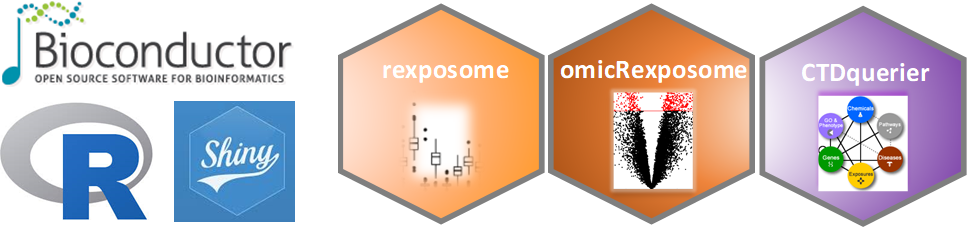
\includegraphics[width=0.6\textwidth,height=\textheight]{images/logo.png}

exposomeShiny is a data analysis toolbox with the following features:

\begin{itemize}
\tightlist
\item
  Data handling: imputation, LOD, transformation, \ldots{}
\item
  Exposome characterization
\item
  Exposome-wide association analysis
\item
  Multivariate association
\item
  Omic data integration
\item
  Omic data association
\item
  Post-omic data analysis: CTD database
\item
  Post-omic data analysis: Enrichment analysis
\end{itemize}

To do so, exposomeShiny relies on previously existent Bioconductor packages (rexposome, omicRexposome and CTDquerier among others), it uses them in a seamless way so the final user of exposomShiny can perform the same studies that would conduct using the Bioconductor packages but without writing a single line of code.

\hypertarget{setup}{%
\chapter{Setup}\label{setup}}

\hypertarget{r-rstudio-and-packages-versions}{%
\section{R, RStudio and Packages Versions}\label{r-rstudio-and-packages-versions}}

If the user chooses to install and use exposomeShiny using RStudio instead of Docker, the list of package versions used for the development of the application is provided for stability purposes. When using the Docker version of the application, all of the following is bundled on the image so the user does not have to deal with the installation of any package.

Software:

\begin{longtable}[]{@{}ll@{}}
\toprule
R software & Version\tabularnewline
\midrule
\endhead
R & 4.0.2\tabularnewline
RStudio & 1.4.1103\tabularnewline
\bottomrule
\end{longtable}

R packages:

\begin{longtable}[]{@{}ll@{}}
\toprule
R Packages & Version\tabularnewline
\midrule
\endhead
shiny & 1.5.0\tabularnewline
shinyBS & 0.61\tabularnewline
rexposome & 1.12.2\tabularnewline
omicRexposome & 1.12.0\tabularnewline
MultiDataSet & 1.18.0\tabularnewline
mice & 3.11.0\tabularnewline
DT & 0.16\tabularnewline
ggplot2 & 3.3.2\tabularnewline
data.table & 1.13.2\tabularnewline
truncdist & 1.0\tabularnewline
shinyalert & 2.0.0\tabularnewline
shinydashboard & 0.7.1\tabularnewline
shinyjs & 2.0.0\tabularnewline
TxDb.Hsapiens.UCSC.hg19.knownGene & 3.2.2\tabularnewline
org.Hs.eg.db & 3.12.0\tabularnewline
GenomicRanges & 1.42.0\tabularnewline
CTDquerier & 1.4.3\tabularnewline
shinycssloaders & 1.0.0\tabularnewline
pastecs & 1.3.21\tabularnewline
shinyWidgets & 0.5.4\tabularnewline
clusterProfiler & 3.18.1\tabularnewline
enrichplot & 1.10.2\tabularnewline
ggupset & 0.3.0\tabularnewline
imputeLCMD & 2.0\tabularnewline
mixOmics & 6.14.0\tabularnewline
\bottomrule
\end{longtable}

There are two different ways of setting up and using exposomeShiny

\hypertarget{downloading-the-source-files-installing-the-libraries-and-running-the-application}{%
\section{Downloading the source files, installing the libraries and running the application}\label{downloading-the-source-files-installing-the-libraries-and-running-the-application}}

The user can choose to download the source code of the shiny application and install all the required libraries on their local R installation. Make sure \href{https://cran.r-project.org/bin/windows/Rtools/history.html}{Rtools} is installed to use this method.

\begin{Shaded}
\begin{Highlighting}[]
  \CommentTok{\# Set working directory}
\FunctionTok{setwd}\NormalTok{(}\AttributeTok{dir =} \StringTok{"/some/path/"}\NormalTok{)}
      
  \CommentTok{\# Download zip}
\FunctionTok{download.file}\NormalTok{(}\AttributeTok{url =} \StringTok{"https://github.com/isglobal{-}brge/exposomeShiny/archive/master.zip"}\NormalTok{, }\AttributeTok{destfile =} \StringTok{"master.zip"}\NormalTok{)}

  \CommentTok{\# Unzip the .zip to the working directory}
\FunctionTok{unzip}\NormalTok{(}\AttributeTok{zipfile =} \StringTok{"master.zip"}\NormalTok{)}

  \CommentTok{\# Set the working directory inside the downloaded folder}
\FunctionTok{setwd}\NormalTok{(}\AttributeTok{dir =} \StringTok{"/some/path/exposomeShiny{-}master"}\NormalTok{)}
\end{Highlighting}
\end{Shaded}

Now all the source files are downloaded to the location of chose and the working directory moved to the correct folder, to start the project, open the \texttt{Rproj} file by clicking it on the Files explorer of RStudio.

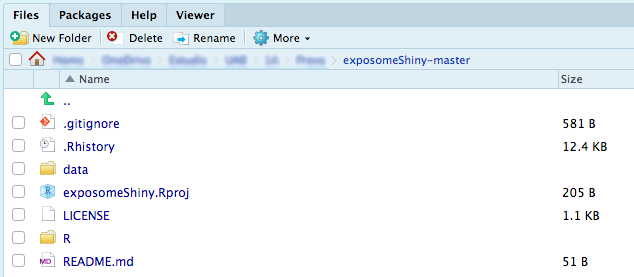
\includegraphics{images/setup1.png}

Once the project is loaded, the file found on the source folder called \texttt{installer.R} has to be sourced and run. This will install the newest versions of the packages required by Exposome Shiny on this R session. To do so, run the following code on the RStudio console.

\begin{Shaded}
\begin{Highlighting}[]
\FunctionTok{source}\NormalTok{(}\StringTok{"installer.R"}\NormalTok{)}
\end{Highlighting}
\end{Shaded}

This is only needed on the first run, once completed it doesn't need to be done prior to launching the application itself any other time.

Now everything is ready to launch the Shiny application. To do so there a two approaches, one is to open the \texttt{ui.R} or the \texttt{server.R} files that are inside the \texttt{R} folder and press \texttt{Run\ App}.

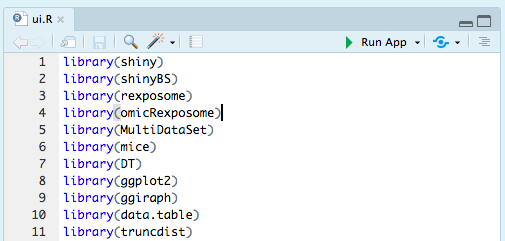
\includegraphics{images/setup2.png}

Or the other option is to input the following command on the console.

\begin{Shaded}
\begin{Highlighting}[]
\NormalTok{shiny}\SpecialCharTok{::}\FunctionTok{runApp}\NormalTok{(}\StringTok{\textquotesingle{}R\textquotesingle{}}\NormalTok{)}
\end{Highlighting}
\end{Shaded}

\hypertarget{pulling-the-official-docker-image-from-dockerhub}{%
\section{Pulling the official Docker image from DockerHub}\label{pulling-the-official-docker-image-from-dockerhub}}

If there's any troubble downloading the required R packages to make exposomeShiny work, there's the option of using Docker. It has the disadvantage of being a little bit difficult to install on a Windows machine, however, it's extremely simple on a Mac OS X / Linux environment. For the Windows users refer to the following links for instructions on how to install Docker and setup you machine to run WSL2 and launch bash commands on Windows \href{https://docs.docker.com/docker-for-windows/install-windows-home/}{1}, \href{https://blog.nillsf.com/index.php/2020/02/17/setting-up-wsl2-windows-terminal-and-oh-my-zsh/}{2}, \href{https://docs.docker.com/docker-for-windows/wsl/}{3}.

To download and launch exposomeShiny, execute the following command on a bash terminal(make sure Docker is running, if not search for the \texttt{Docker\ Desktop} app and launch it).

\begin{Shaded}
\begin{Highlighting}[]
\ExtensionTok{docker}\NormalTok{ run {-}{-}rm {-}p 80:80 brgelab/exposome{-}shiny}
\end{Highlighting}
\end{Shaded}

This command will download the Docker image of exposomeShiny (be aware it weights \textasciitilde{} 3 GB, so if your internet connection is slow it may take a while) and run a container with it. The container will be exposed on the local port 80 and it will render on that port the application itself, so to start using exposomeShiny open your web browser and go to the site

\begin{Shaded}
\begin{Highlighting}[]
\ExtensionTok{localhost}\NormalTok{:80}
\end{Highlighting}
\end{Shaded}

At the beginning it may take some time for the application to render, this is because all the needed R libraries are being loaded, to be sure the container is actually working, take a look at the terminal where you inputed the Docker command, there you will see all the R verbose stating the libraries are being loaded.

Once the user has finished using exposomeShiny, the container needs to be stopped to avoid wasting CPU resources, to do so, input the following command on a bash terminal (the command needs to be inputed on a new bash window):

\begin{Shaded}
\begin{Highlighting}[]
\ExtensionTok{docker}\NormalTok{ container ls}
\end{Highlighting}
\end{Shaded}

This will prompt all the running containers, find the one with the NAMES \texttt{brgelab/exposome-shiny} and copy it's CONTAINER ID, then input the following bash command:

\begin{Shaded}
\begin{Highlighting}[]
\ExtensionTok{docker}\NormalTok{ stop xxxxxxxxxxxx}
\end{Highlighting}
\end{Shaded}

Where xxxxxxxxxxxx is the CONTAINER ID.

To run the application again, just enter the first bash command (\texttt{docker\ run\ -\/-rm\ -p\ 80:80\ brgelab/exposome-shiny}), since it has already been downloaded, the application is cached on the computer and it will launch straight away. If the user wants to remove the Docker image from the computer, input the following bash command:

\begin{Shaded}
\begin{Highlighting}[]
\ExtensionTok{docker}\NormalTok{ image rm brgelab/exposome{-}shiny}
\end{Highlighting}
\end{Shaded}

\hypertarget{data-sets}{%
\chapter{Data sets}\label{data-sets}}

\hypertarget{expo_data}{%
\section{Exposome dataset}\label{expo_data}}

The exposome is composed of three different files (in \texttt{*.csv}, \texttt{*.tsv} or \texttt{*.txt} format). Those files are refered inside the Shiny as exposures, description and phenotypes. Their content is the following:

\begin{itemize}
\tightlist
\item
  The \texttt{exposures} file contains the measures of each exposure for all the individuals included on the analysis. It is a matrix-like file having a row per individual and a column per exposures. It must includes a column with the subject's identifier.
\item
  The \texttt{description} file contains a row for each exposure and, at last, defined the families of exposures. Usually, this file incorporates a description of the exposures, the matrix where it was obtained and the units of measurement among others.
\item
  The \texttt{phenotypes} file contains the covariates to be included in the analysis as well as the health outcomes of interest. It contains a row per individual included in the analysis and a column for each covariate and outcome. Moreover, it must include a column with the individual's identifier.
\end{itemize}

Some remarks regarding this files:

\begin{itemize}
\tightlist
\item
  All three files have to share the same separator element, for \texttt{*.csv} files is typical to use a comma (,) but it could also be a semicolon (;).
\item
  The exposure names have to start with a character {[}a-z/A-Z{]}, leading special characters will cause the data entry to return errors.
\item
  Exactly the same exposures have to be present on the description and exposures files.
\item
  Exactly the same samples have to be present on the exposures and phenotypes files.
\item
  The exposures and phenotypes files have an ID column, the description file does not have an ID column nor row.
\end{itemize}

A visual representation of the three matrices and how they correlate is the following.

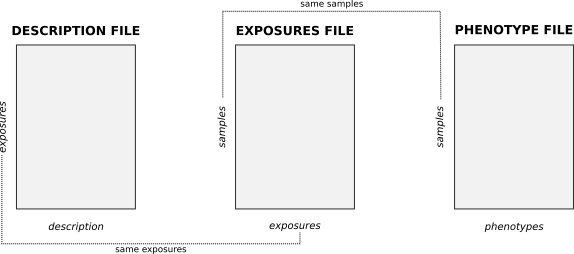
\includegraphics{images/exposome_dataset_struct.png}

Exposures data file example:

\begin{verbatim}
id    bde100  bde138  bde209  PFOA    ...
sub01  2.4665  0.7702  1.6866  2.0075 ...
sub02  0.7799  1.4147  1.2907  1.0153 ...  
sub03 -1.6583 -0.9851 -0.8902 -0.0806 ... 
sub04 -1.0812 -0.6639 -0.2988 -0.4268 ... 
sub05 -0.2842 -0.1518 -1.5291 -0.7365 ... 
...   ...     ...     ...     ...
\end{verbatim}

Description data file example:

\begin{verbatim}
exposure  family  matrix         description
bde100    PBDEs   colostrum       BDE 100 - log10
bde138    PBDEs   colostrum       BDE 138 - log10
bde209    PBDEs   colostrum       BDE 209 - log10
PFOA      PFAS    cord blood      PFOA - log10
PFNA      PFAS    cord blood      PFNA - log10
PFOA      PFAS    maternal serum  PFOA - log10
PFNA      PFAS    maternal serum  PFNA - log10
hg        Metals  cord blood      hg - log 10
Co        Metals  urine           Co (creatinine) - log10
Zn        Metals  urine           Zn (creatinine) - log10
Pb        Metals  urine           Pb (creatinine) - log10
THM       Water   ---             Average total THM uptake - log10
CHCL3     Water   ---             Average Chloroform uptake - log10
BROM      Water   ---             Average Brominated THM uptake - log10
NO2       Air     ---             NO2 levels whole pregnancy- log10
Ben       Air     ---             Benzene levels whole pregnancy- log10
\end{verbatim}

Phenotypes data file example:

\begin{verbatim}
id    asthma   BMI      sex  age  ...
sub01 control  23.2539  boy  4    ...
sub02 asthma   24.4498  girl 5    ...
sub03 asthma   15.2356  boy  4    ...
sub04 control  25.1387  girl 4    ...
sub05 control  22.0477  boy  5    ...
...   ...      ...      ...  ...
\end{verbatim}

\hypertarget{plain_data_expl}{%
\section{Plain datasets}\label{plain_data_expl}}

If the researcher has gathered all the data on a single file which contains both phenotype and exposure data, this file can be used too. The user interface has a selector for it, more information on the \protect\hyperlink{plain_data}{correspondent section}.

A visual representation of a plain dataset is the following.

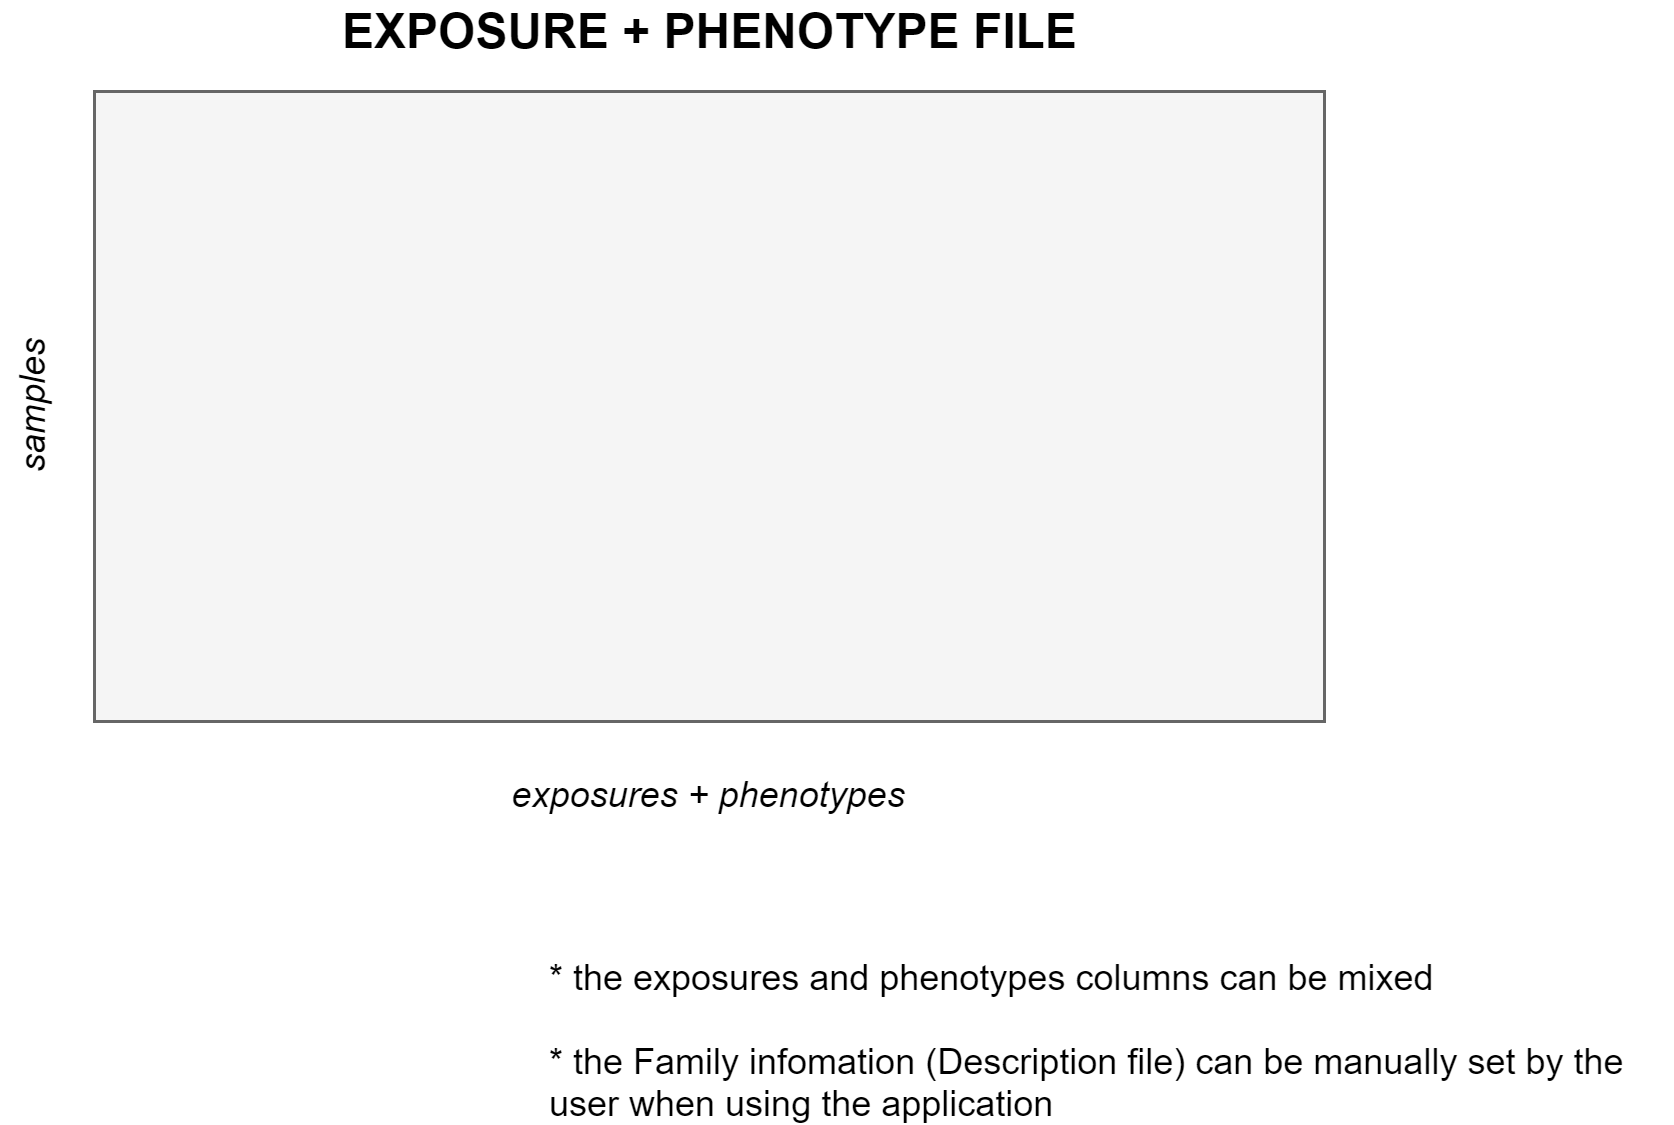
\includegraphics{images/plain_tables.png}

Plain dataset example (3 exposures + 2 phenotypes):

\begin{verbatim}
id    bde100  bde138  bde209    asthma   BMI      ...
sub01  2.4665  0.7702  1.6866   control  23.2539  ...
sub02  0.7799  1.4147  1.2907   asthma   24.4498  ...  
sub03 -1.6583 -0.9851 -0.8902   asthma   15.2356  ... 
sub04 -1.0812 -0.6639 -0.2988   control  25.1387  ... 
sub05 -0.2842 -0.1518 -1.5291   control  22.0477  ...
...   ...     ...      ...      ...      ...
\end{verbatim}

\hypertarget{omicsds}{%
\section{Omics dataset}\label{omicsds}}

The omics data inputed to the Shiny must be provided as an \texttt{*.RData}. This file has to contain an ExpressionSet, which is an S4 object. This object is a data container of the Bioconductor toolset.

For further information on ExpressionSet and how to create and manipulate them, please visit the \href{https://www.bioconductor.org/packages/devel/bioc/vignettes/Biobase/inst/doc/ExpressionSetIntroduction.pdf}{official documentation} and this \href{https://kasperdanielhansen.github.io/genbioconductor/html/ExpressionSet.html}{selected vignette}.

\hypertarget{bioconductor-packages}{%
\chapter{Bioconductor packages}\label{bioconductor-packages}}

This Shiny application is a front end support for other Bioconductor packages in order to provide a comfortable environment on to conduct different analysis with those packages. In concrete the packages are \href{https://www.bioconductor.org/packages/release/bioc/html/rexposome.html}{rexposome}, \href{https://bioconductor.org/packages/release/bioc/html/omicRexposome.html}{omicRexposome} and \href{http://www.bioconductor.org/packages/release/bioc/html/CTDquerier.html}{CTDquerier}.

\hypertarget{rexposome}{%
\section{rexposome}\label{rexposome}}

Rexposome is a package that allows to explore the exposome and to perform association analyses between exposures and health outcomes.

\hypertarget{omicrexposome}{%
\section{omicRexposome}\label{omicrexposome}}

OmicRexposome is a package that systematizes the association evaluation between exposures and omic data, taking advantage of MultiDataSet for coordinated data management, rexposome for exposome data definition and limma for association testing. Also to perform data integration mixing exposome and omic data using multi co-inherent analysis (omicade4) and multi-canonical correlation analysis (PMA).

\hypertarget{ctdquerier}{%
\section{CTDquerier}\label{ctdquerier}}

CTDquerier is a package to retrieve and visualize data from the \href{http://ctdbase.org/}{Comparative Toxicogenomics Database}. The downloaded data is formated as DataFrames for further downstream analyses.

\hypertarget{analysis-flowcharts}{%
\chapter{Analysis flowcharts}\label{analysis-flowcharts}}

On this section, a detailed guide on how to perform different analyses using exposomeShiny will be provided. The guide contains screenshots of the analysis steps as well as some flowcharts.

\hypertarget{exposome-health-analysis}{%
\section{Exposome health analysis}\label{exposome-health-analysis}}

The exposome health analysis corresponds to the study of the relation between exposures (exposome) and health outcomes (phenotypes). Information about exposome data exploration and pre-processing can also be found on this subsection. Along this section, the data files used as examples are: \texttt{exposures.csv}, \texttt{exposures\_lod.csv}, \texttt{description.csv}, \texttt{phenotypes.csv} and \texttt{exposome\_plain.csv} which are available \href{https://github.com/isglobal-brge/exposomeShiny/tree/master/data}{here}.

\hypertarget{data-entry}{%
\subsection{Data entry}\label{data-entry}}

There are two different data entry methods. \protect\hyperlink{expo_data}{Exposome data} which uses the three tables and \protect\hyperlink{plain_data_expl}{plain data} which only uses one.

\hypertarget{exposome-data}{%
\subsubsection{Exposome data}\label{exposome-data}}

Three tables are needed to input an exposome dataset: the exposures, description and phenotypes. This files have to be provided as \texttt{csv} or \texttt{txt}. Different separator formats are supported (`,', `;', tabs and spaces). Excel files or R objects are not supported as inputs. Be sure all three files share the same separator.

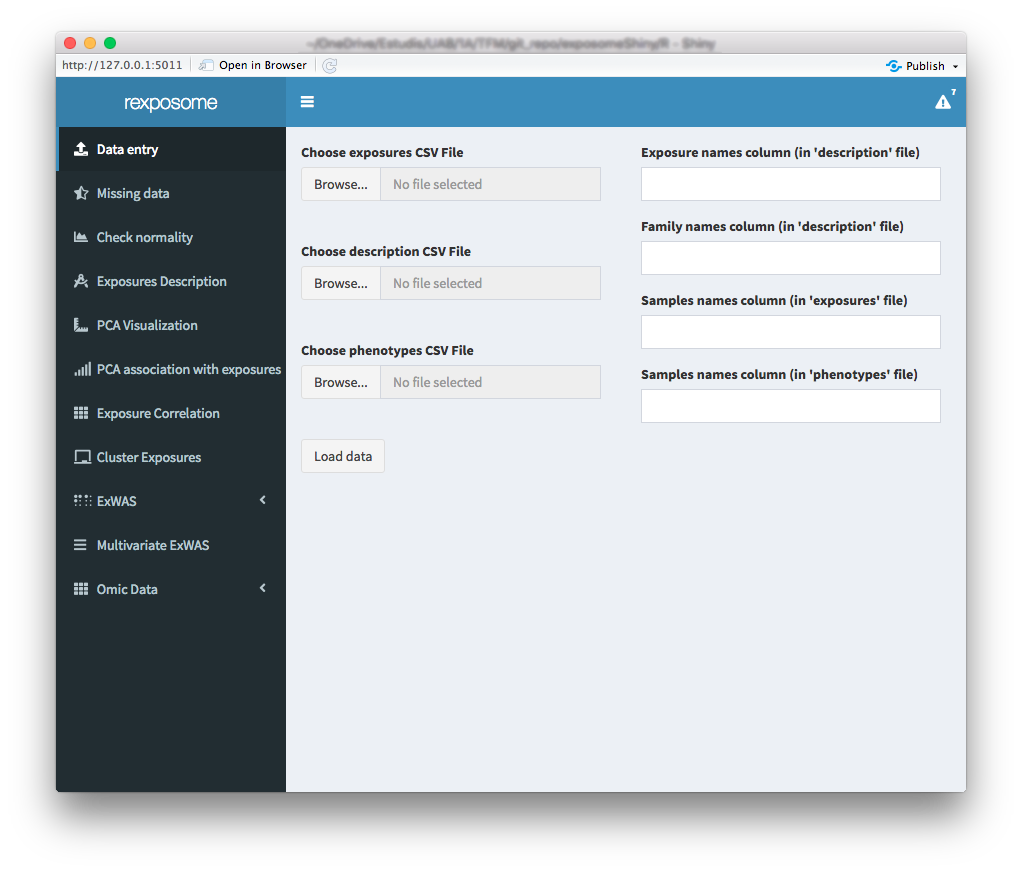
\includegraphics{images/analysis1_2.png}

Once the tables are read two new main elements will appear, 1) the option to explore the inputted tables; and 2) six input fields which control the following file parameters:

\begin{itemize}
\tightlist
\item
  Column name in the \emph{description} file that contains the exposures
\item
  Column name in the \emph{description} file that contains the families
\item
  Column name in the \emph{exposures} file that contains the identifier
\item
  Column name in the \emph{phenotypes} file that contains the identifier
\item
  The threshold to select between continuous or factor exposures. More than this number of unique items on an exposure will be considered as `continuous'
\item
  The encoding to search for limit of detection (LOD) missings. It can be either a number (example: \texttt{-1}) or a string (example: \texttt{LOD}). All the cells that contain this encoder will be considered LOD missings.
\end{itemize}

This is illustrated on the following figure.

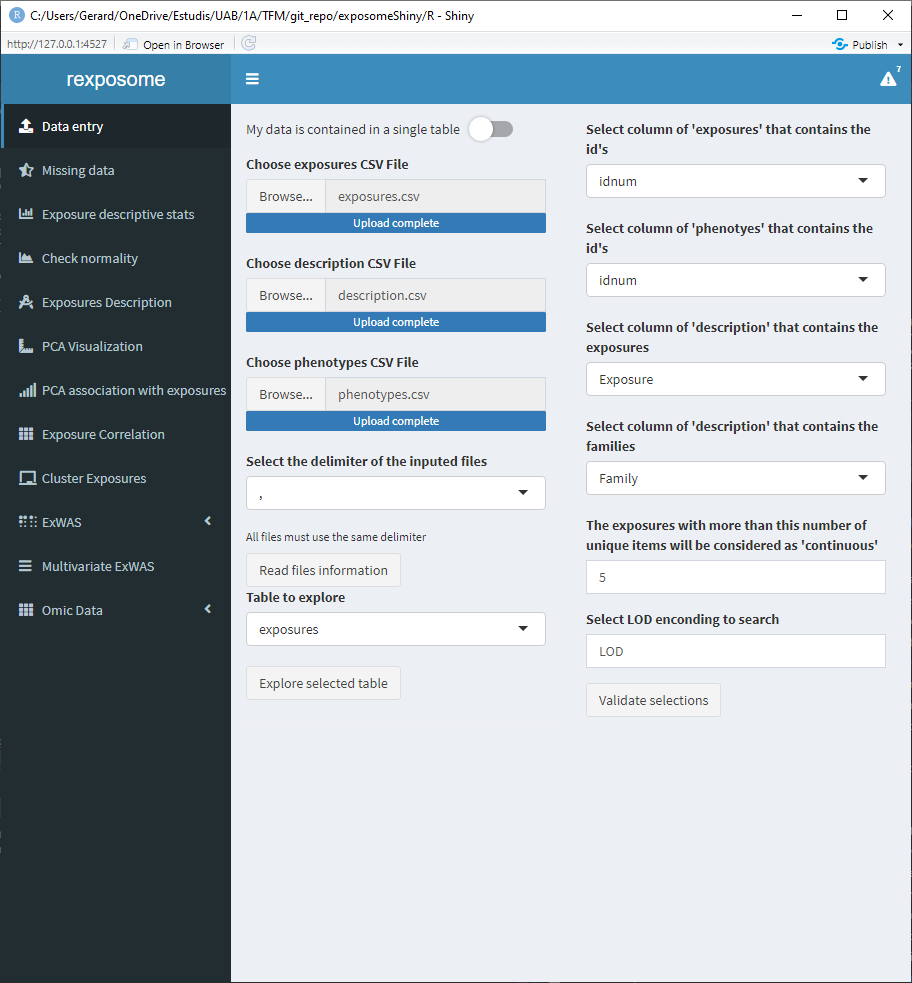
\includegraphics{images/analysis1_2_2.png}

Once the fields are completed, press the \emph{Validate selections} button in order to check if all the parameters allow for a successful load of the exposome dataset, if not, a pop-up will be prompted to the user with the R error message that stopped the execution. In the case that everything is correct, the interface will be updated and a button that reads \emph{Load selected data to analyze it} will appear, by clicking this button the dataset will be loaded.

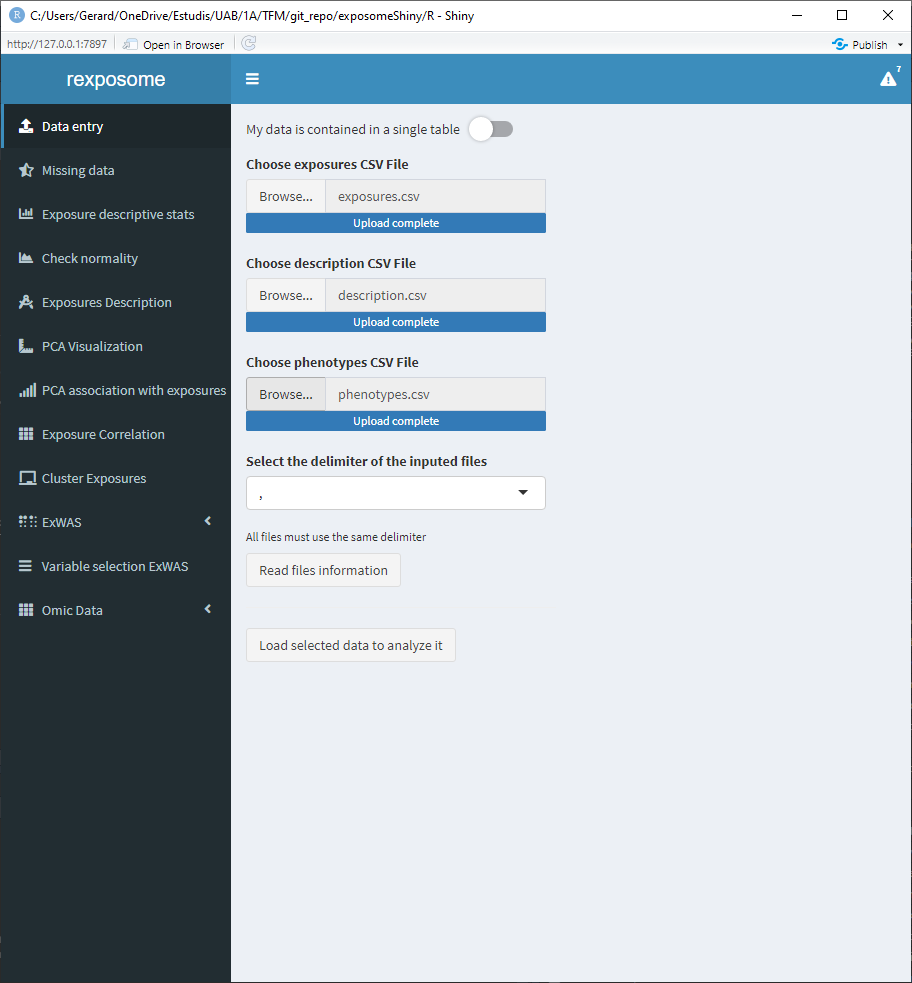
\includegraphics{images/analysis1_2_2_1.png}

\hypertarget{plain_data}{%
\subsubsection{Plain data}\label{plain_data}}

When dealing with a single file that contains the exposures and phenotype data, press the ``My data is contained in a single table'' toggle. This will change the interface to only show one file selector.

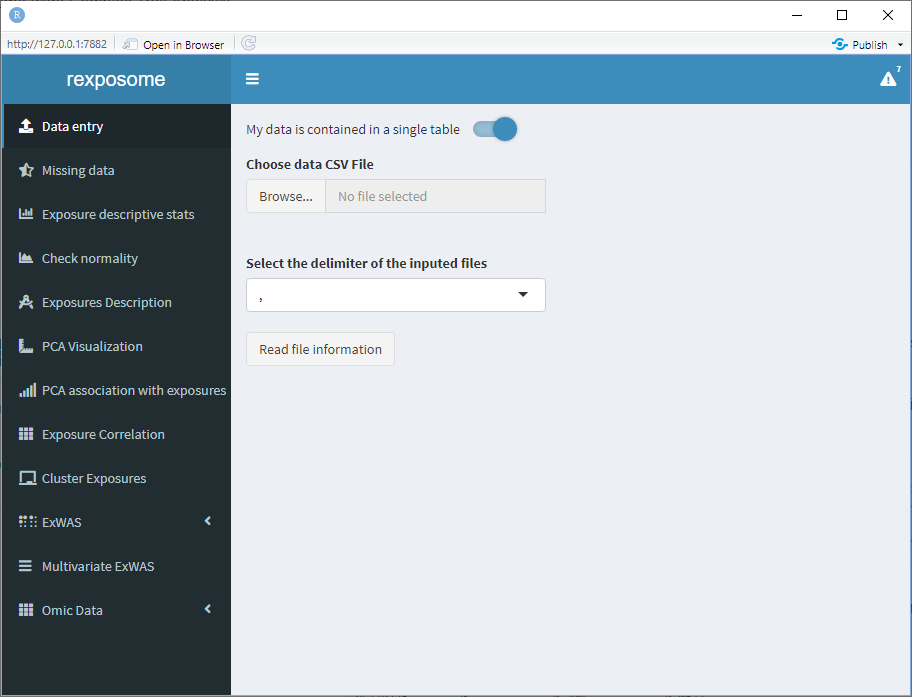
\includegraphics{images/plain_table_1.png}

Select a file and press ``Read file information''. This will change the interface to show a multiple selector input, all the available columns will be listed, select the ones which correspond to phenotypes.

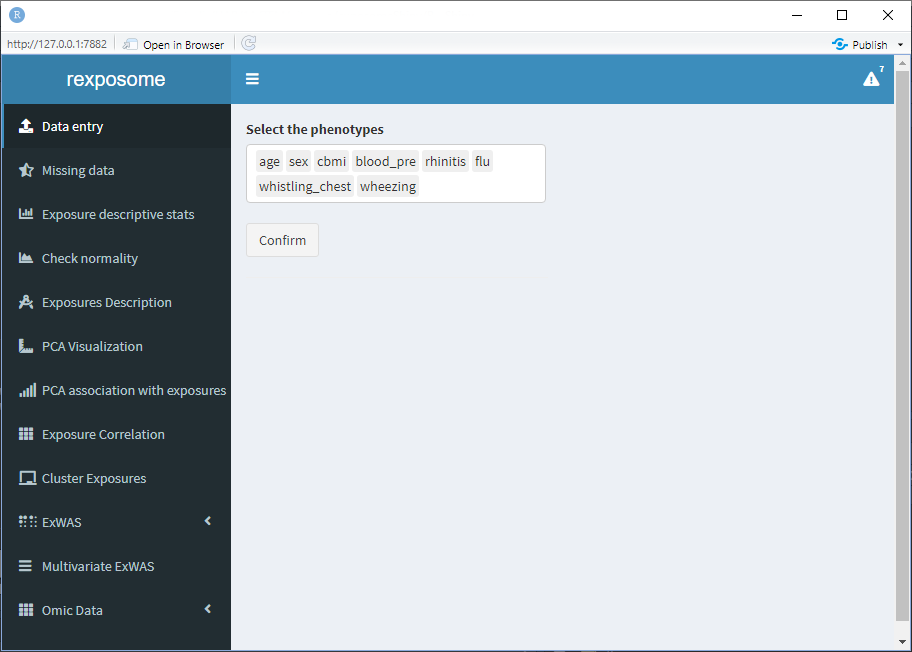
\includegraphics{images/plain_table_2.png}

When all the phenotypes are selected, press ``Confirm''. Now the exposures can be grouped into families, to do so:

\begin{itemize}
\tightlist
\item
  Select all the exposures from the same family
\item
  Write the family name on the box ``Family of selected exposures''
\item
  Press the ``Assign'' button
\end{itemize}

The table will be updated to visualize the action performed.

Exposures left with an empty ``Family'' field will be treated as they are their own family.

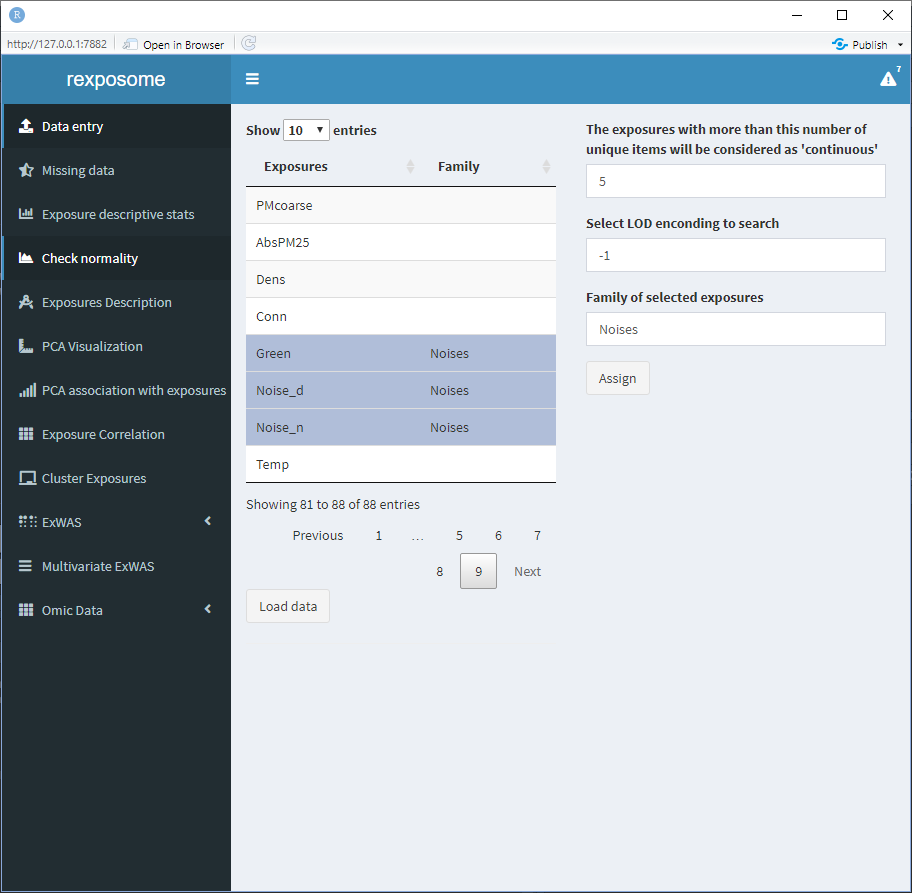
\includegraphics{images/plain_table_3.png}

Finally, there are two configuration fields:

\begin{itemize}
\tightlist
\item
  The threshold to select between continuous or factor exposures. More than this number of unique items on an exposure will be considered as `continuous'
\item
  The encoding to search for limit of detection (LOD) missings (example: \texttt{LOD}). All the cells that contain this encoder will be considered LOD missings.
\end{itemize}

Be sure to revise them before pressing ``Load data''.

\hypertarget{lod-imputation}{%
\subsection{LOD imputation}\label{lod-imputation}}

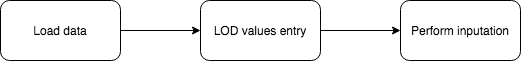
\includegraphics{images/analysis1_1.png}

When loading the data, if LOD missings are detected a small table with the exposures that have LOD missings will appear at the bottom of the ``Data entry'' page.

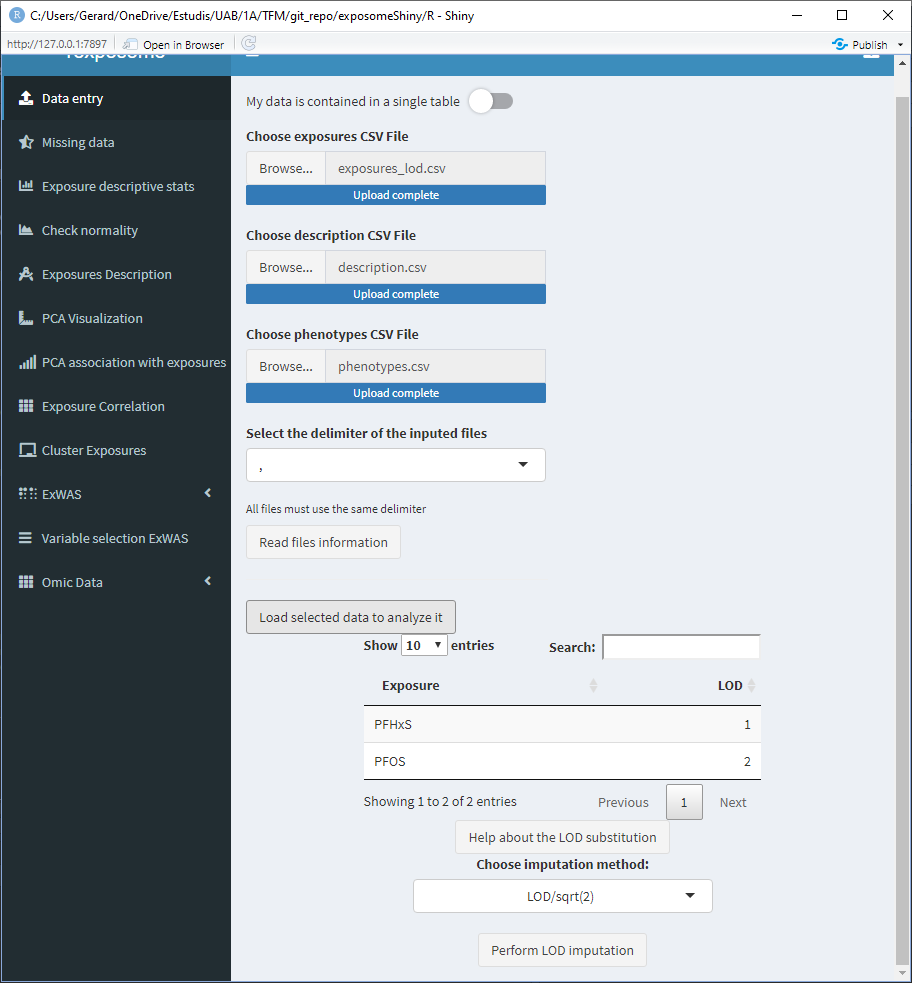
\includegraphics{images/analysis1_2_3.png}

This table has a column named ``LOD'', which by default reads as 1, 2, 3, \ldots{} Those values are meant to be modified by the user and input the limit of detection values for the different exposures. Those values will be used if the LOD imputation method is LOD/sqrt(2). If the imputation method used is QRILC there is no need to modify those values, as they won't be used.

To modify the LOD values of the table, double click on the cell of interest and type the value (use points for decimal separation e.j. 1.156).

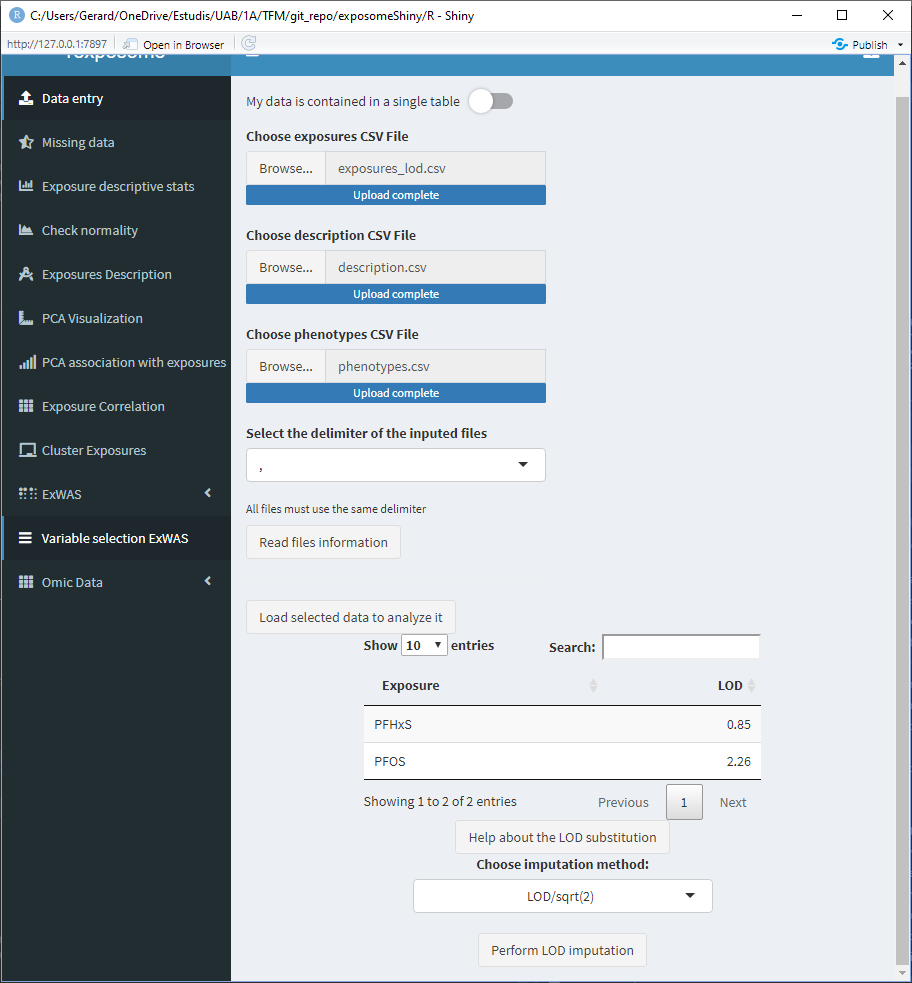
\includegraphics{images/analysis1_2_4.png}

After clicking ``Perform LOD imputation'', a new button to download the imputed dataset will appear, this will download the exposures data with the LOD missings imputed.

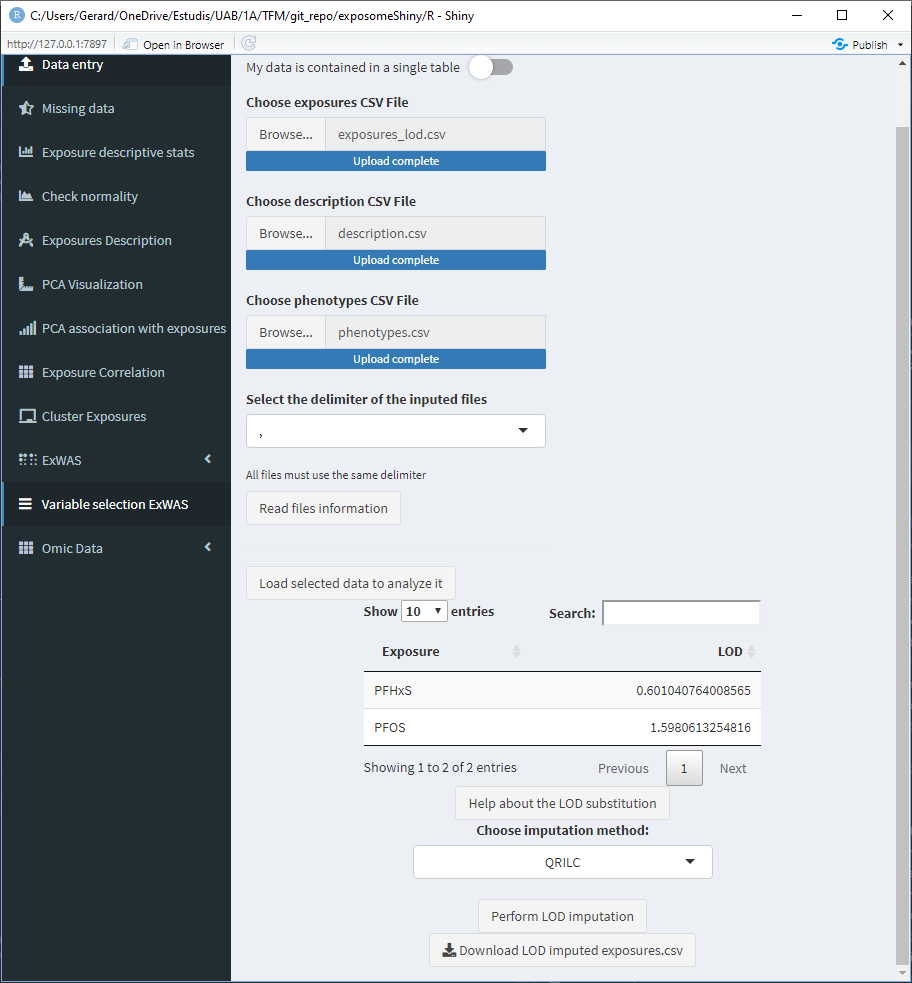
\includegraphics{images/analysis1_2_5.png}

Once the LOD imputation is completed, the exposome dataset that will be used on the following steps is imputed.

\hypertarget{missing-imputation}{%
\subsection{Missing imputation}\label{missing-imputation}}

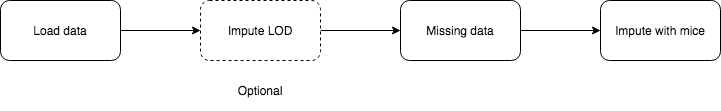
\includegraphics{images/analysis2_1.png}

The ``Missing data'' tab displays a plot with the percentages of missing data for each exposure.

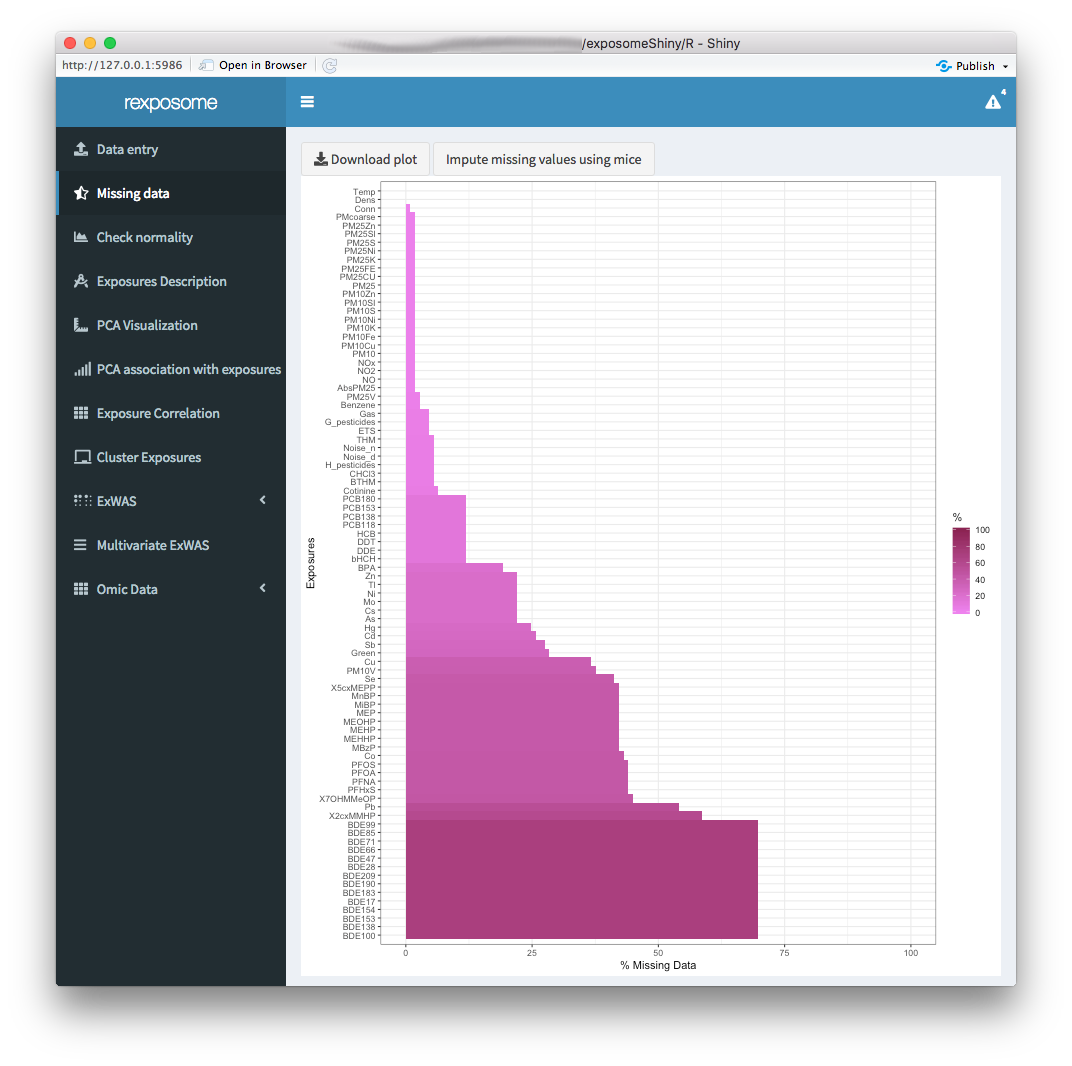
\includegraphics{images/analysis2_2.png}

The missings can be imputed using Multiple Imputation by Chained Equations (MICE) by clicking the ``Impute missing values using mice'' button.

Please note that missings imputation might require other methodologies or more fine control. If that is the case, we encourage users to impute the data beforehand and input to our application data that is already imputed.

Once the missings imputation is completed, the exposome dataset that will be used on the following steps is imputed. This is reflected by refreshing the plot, which should read 0\% missings for all exposures.

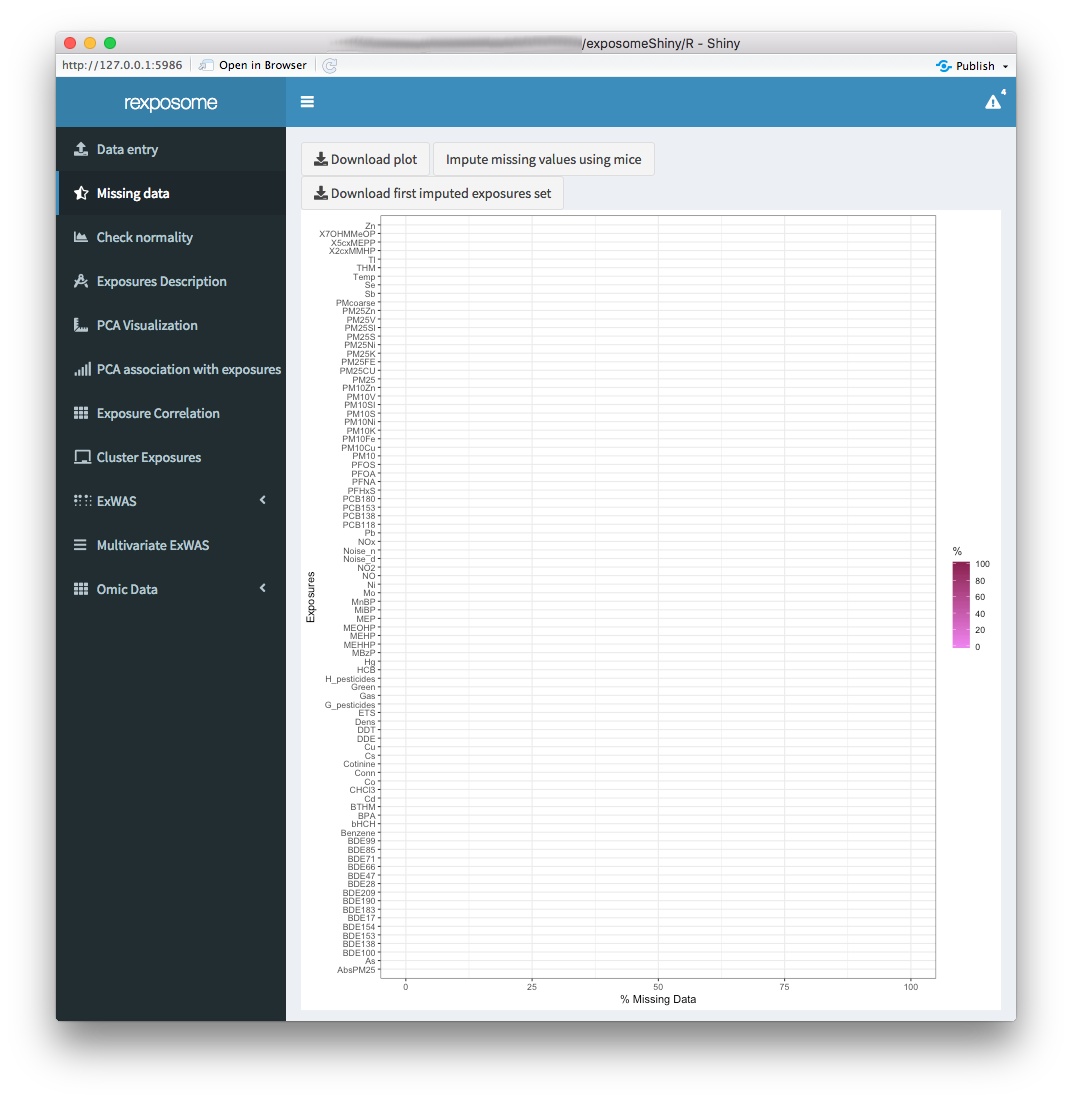
\includegraphics{images/analysis2_3.png}

The imputed exposures set can be downloaded as a \texttt{*.csv} file.

\hypertarget{exposures-description}{%
\subsection{Exposures description}\label{exposures-description}}

The exposure descriptive stats tab, provides a table with the main descriptive stats of the quantitative exposures. The descriptive stats (per exposure) included on the table are:

\begin{itemize}
\tightlist
\item
  Number of values
\item
  Number of NULLs
\item
  Number of NAs
\item
  Minimum
\item
  Maximum
\item
  Range of values
\item
  Sum of values
\item
  Median
\item
  Mean
\item
  Standard Error of mean
\item
  0.95 confidence interval of the mean
\item
  Variance
\item
  Standard deviation
\item
  Variance coefficient
\end{itemize}

Remember that after imputing the missings, the imputed dataset becomes active, this will be reflected showing 0 NAs for example.

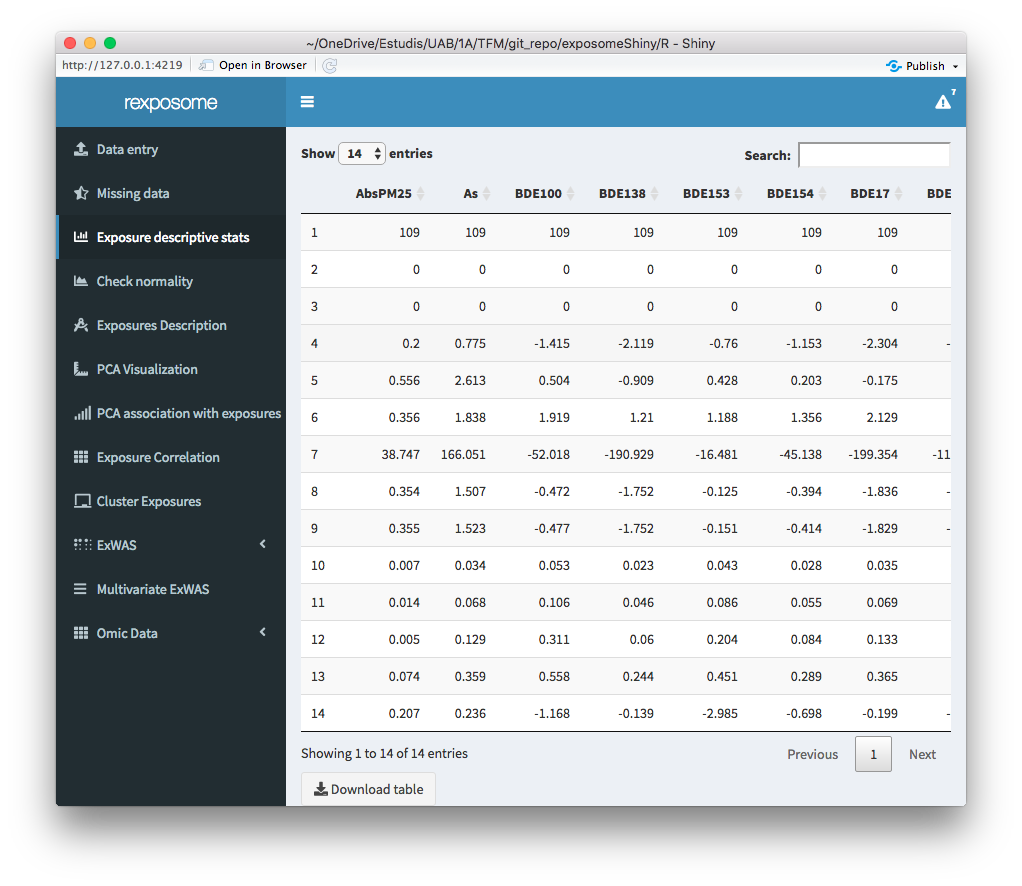
\includegraphics{images/analysis2_4.png}

\hypertarget{normality-correction}{%
\subsection{Normality correction}\label{normality-correction}}

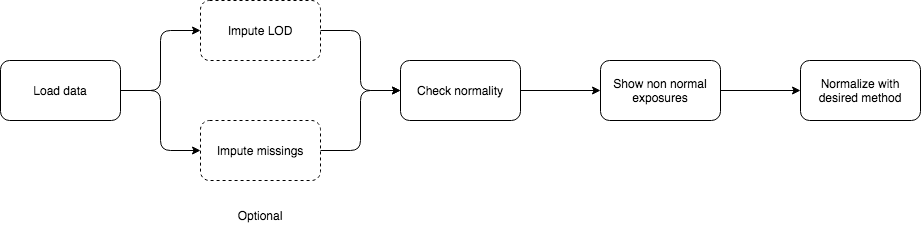
\includegraphics{images/analysis3_1.png}

The table shown on the `Check normality' tab contains all the exposures, if they can be considered normal distributed and the p-value of the normality test (Shapiro-Wilk).

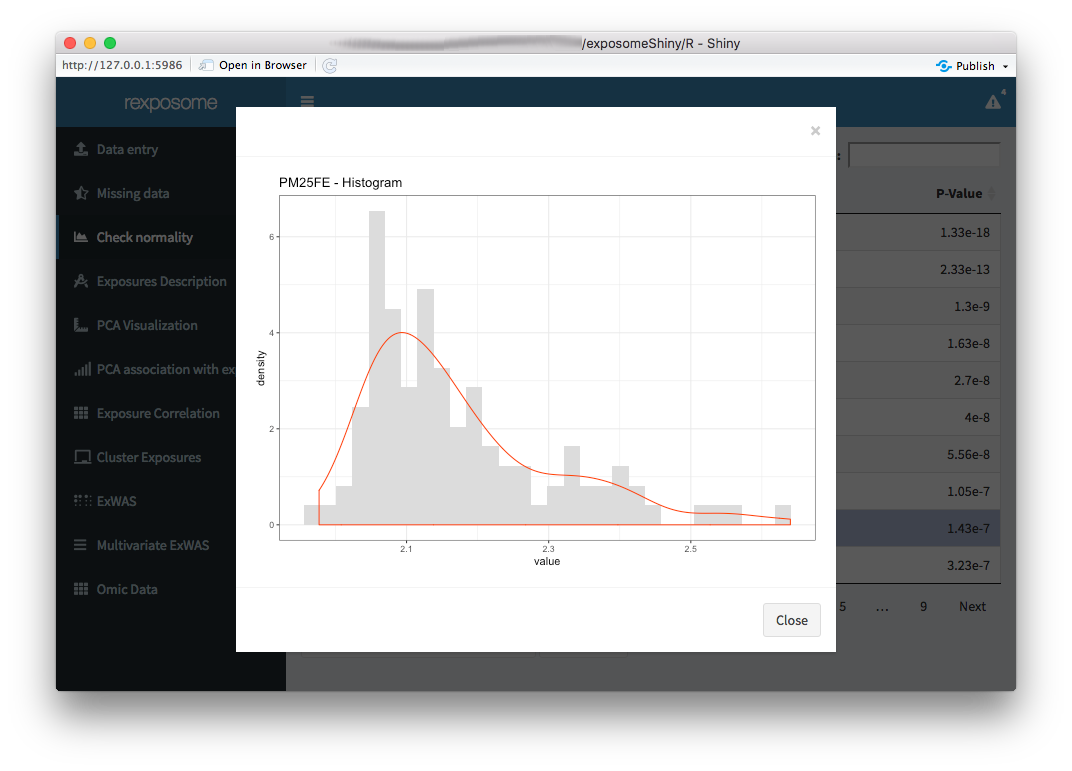
\includegraphics{images/analysis3_2.png}

Select an exposure from the table and click on `Plot histogram of selected exposure' to see the histogram of that exposure.

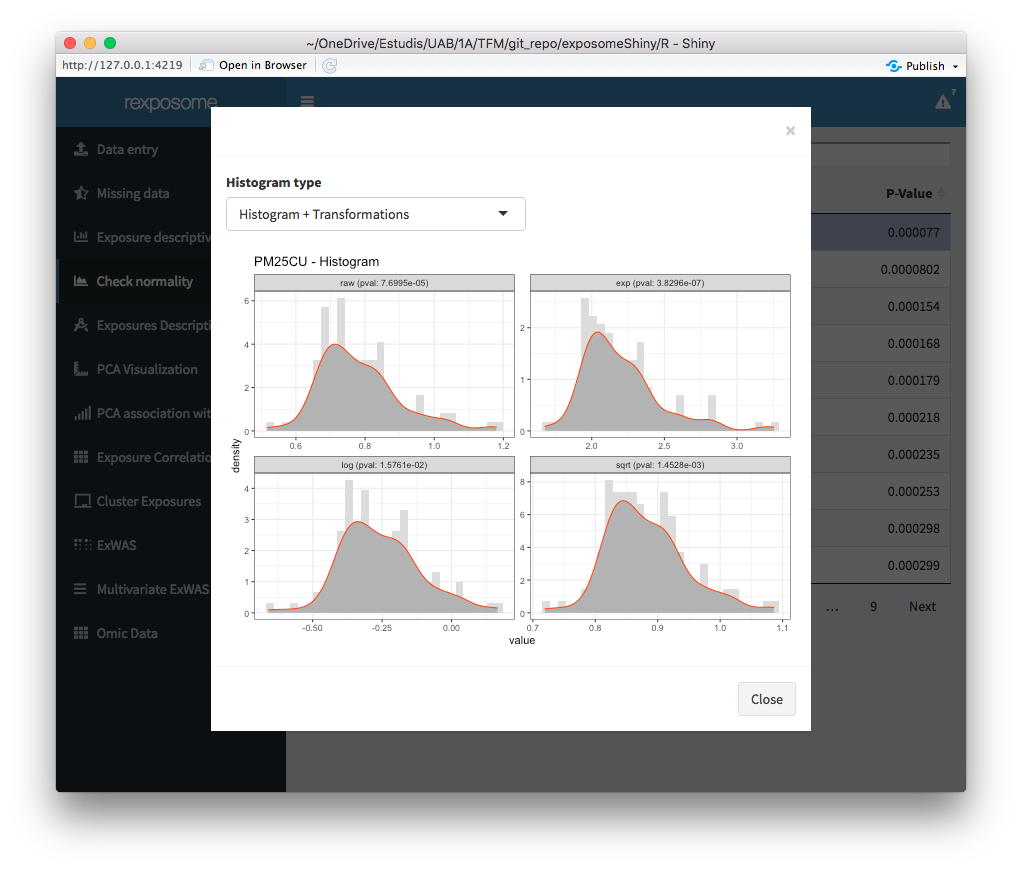
\includegraphics{images/analysis3_2_2.png}

There is the option to visualize the histograms with the available transformations applied, in order to see how an exposure will be affected by them. To see it select `Histogram + transformations' on the Histogram type.

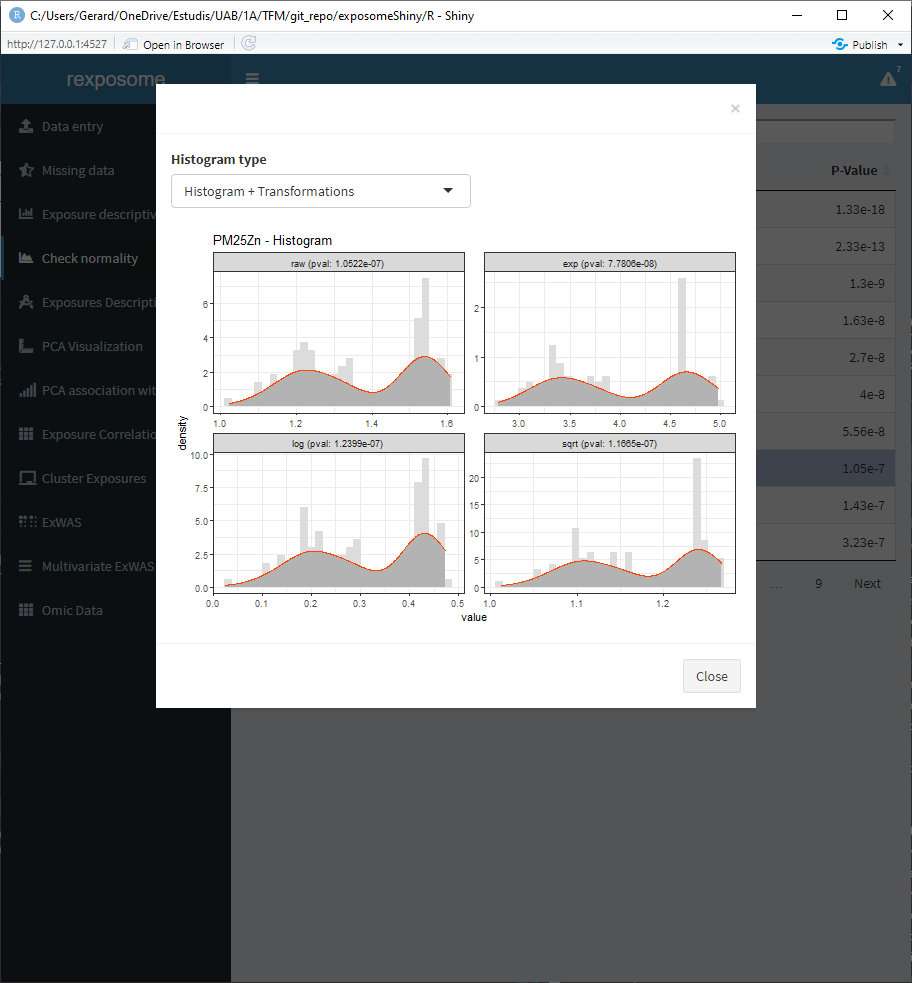
\includegraphics{images/analysis3_2_3.png}

Aside from visualizing if exposures are normal, this tab can be used to apply transformations to the exposures. The available transformations are ``log'' (default, natural logarithm), ``\^{}1/3'' and ``sqrt''. To do so, the procedure is the following:

\begin{itemize}
\tightlist
\item
  Press the `Show false' button. A pop-up will appear with a table. This table contains all the exposures that did not pass the normality test, next to the exposures the transformation to be applied is shown.
\end{itemize}

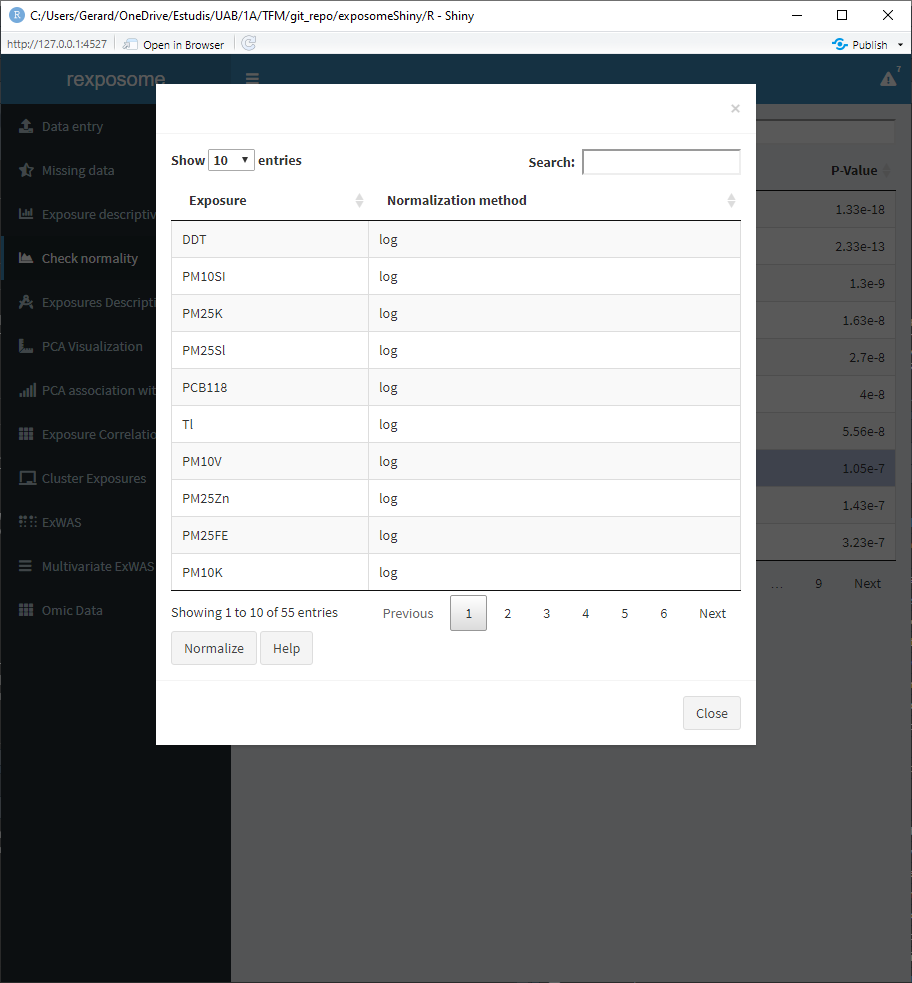
\includegraphics{images/analysis3_3.png}

\begin{itemize}
\tightlist
\item
  Modify the transformation method by double clicking on the cell to be changed and typing the required method. Input `none' if no transformation is desired for a certain exposure.
\end{itemize}

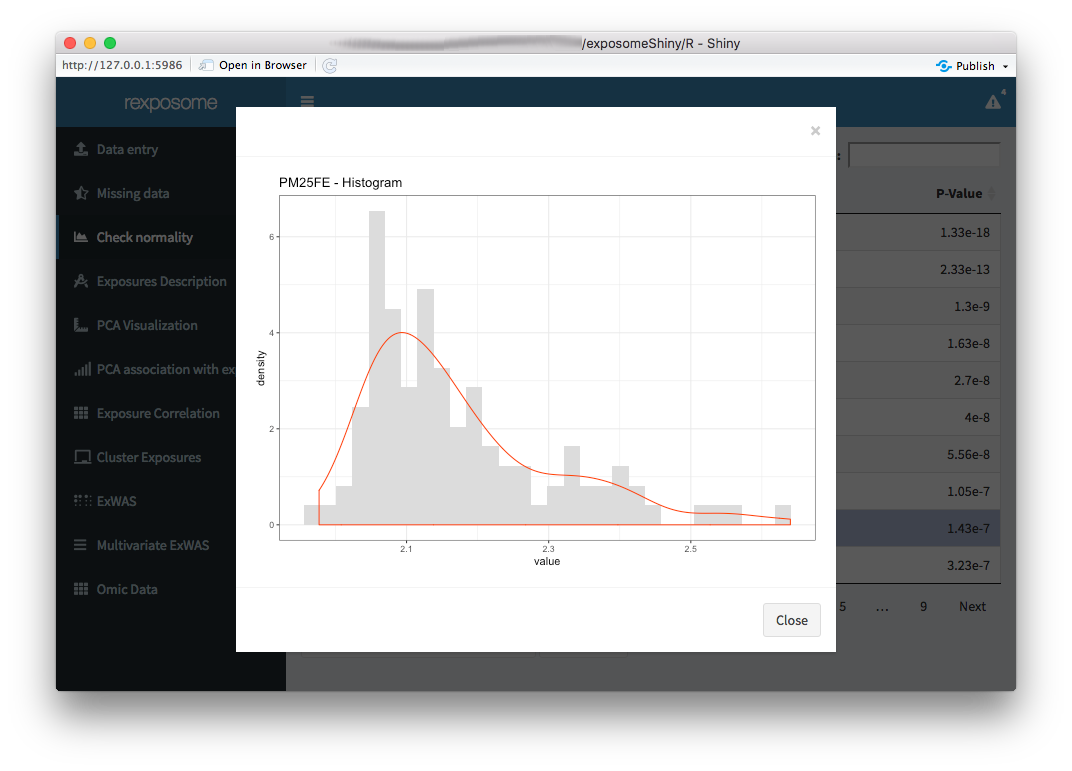
\includegraphics{images/analysis3_2.png}

\begin{itemize}
\tightlist
\item
  Press `Normalize' to apply the transformations.
\end{itemize}

After the transformations are applied, the table of normality tests will be updated. The dataset used after transforming is updated with the new values.

\hypertarget{exposures-description-1}{%
\subsection{Exposures description}\label{exposures-description-1}}

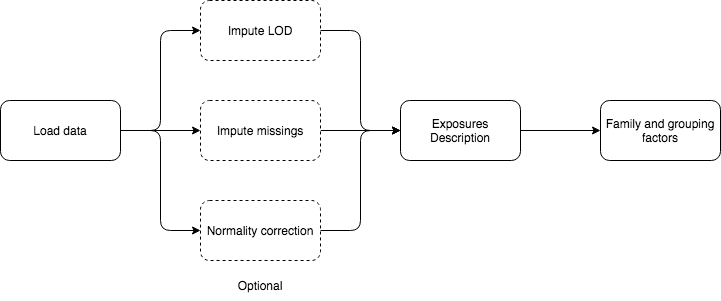
\includegraphics{images/analysis4_1.png}

On the `Exposures description' tab, exploratory analysis of the exposures can be performed. Again, the data analyzed by this tab will be imputed or normalized if the user has performed it before.

There are three input fields to obtain different plots:

\begin{itemize}
\tightlist
\item
  Family: To define which family of exposures wil be plotted
\item
  Grouping factor: Qualitative phenotype to group the exposures
\item
  Second grouping factor: Second qualitative phenotype to group the exposures
\end{itemize}

The visualization is different for categorical and quantitative exposures.

Some examples:

\hypertarget{quantitative-family-grouped-by-sex}{%
\subsubsection{Quantitative family, grouped by sex}\label{quantitative-family-grouped-by-sex}}

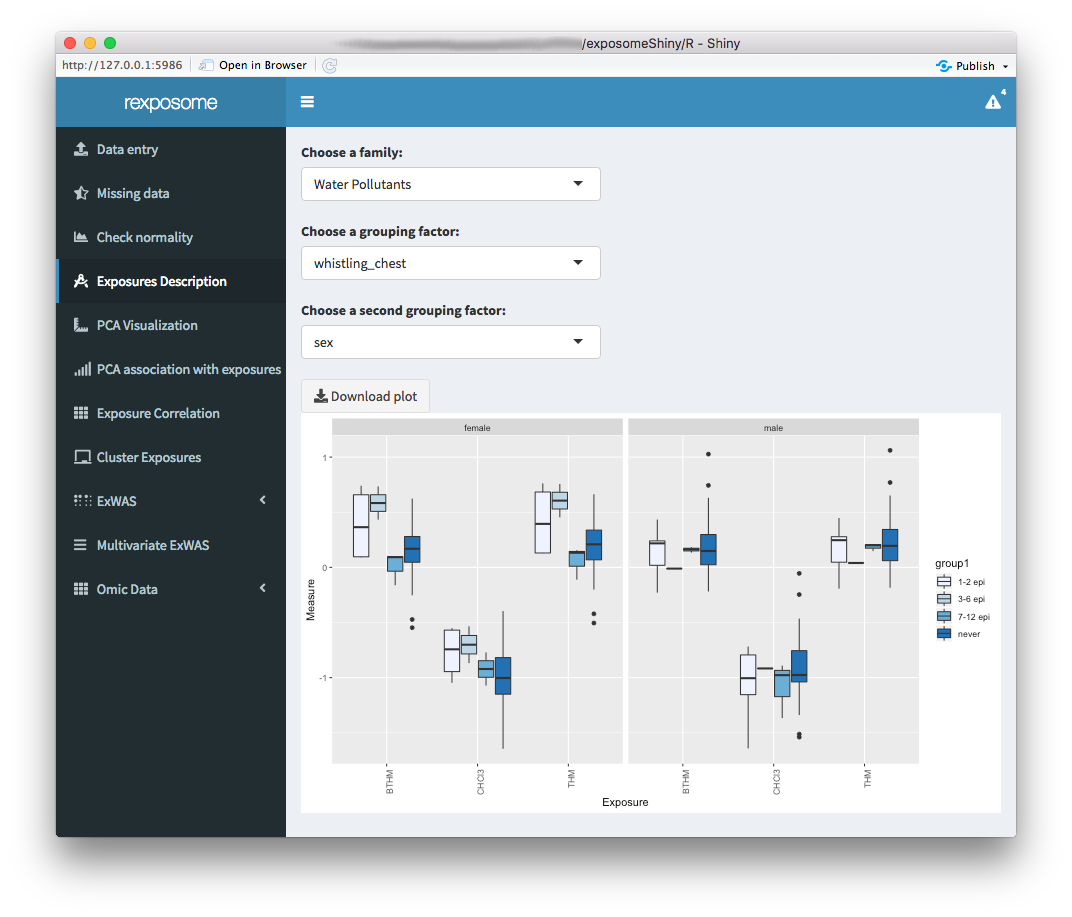
\includegraphics{images/analysis4_2.png}

\hypertarget{qualitative-family-grouped-by-sex}{%
\subsubsection{Qualitative family, grouped by sex}\label{qualitative-family-grouped-by-sex}}

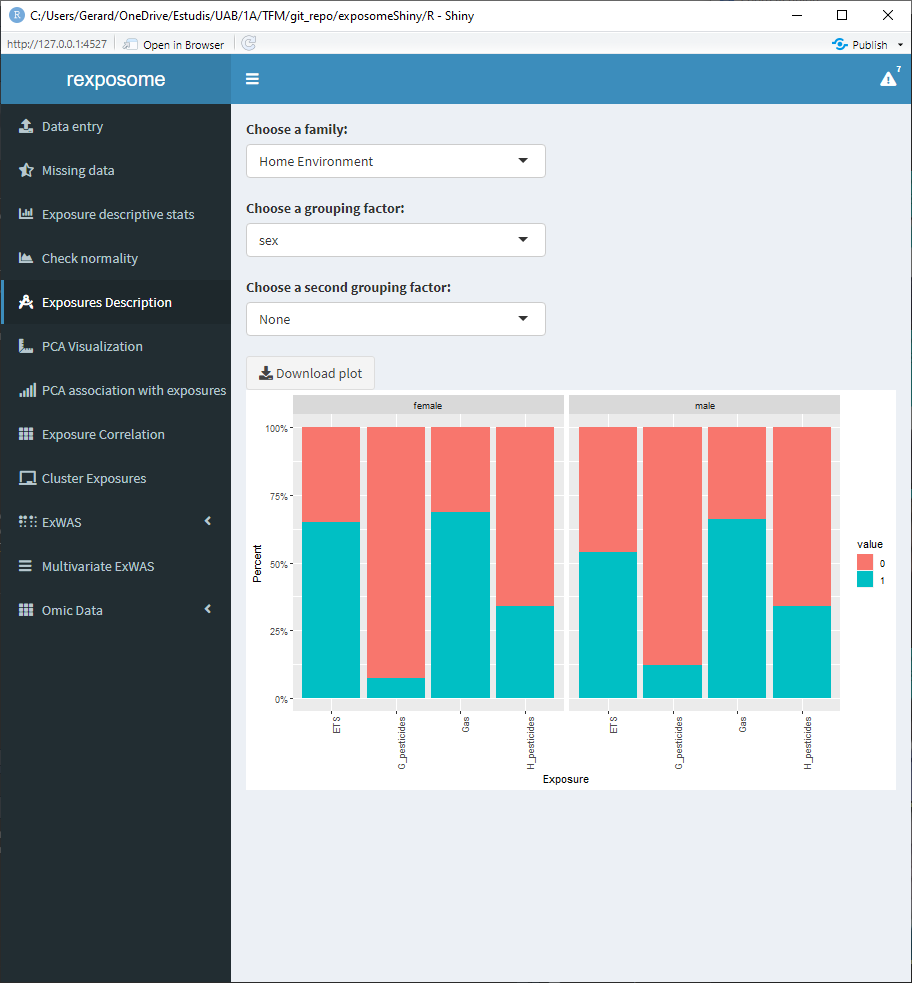
\includegraphics{images/analysis4_2_1.png}

\hypertarget{quantitative-family-grouped-by-sex-and-flu-diagnosis-binomial-factor}{%
\subsubsection{Quantitative family grouped by sex and flu diagnosis (binomial factor)}\label{quantitative-family-grouped-by-sex-and-flu-diagnosis-binomial-factor}}

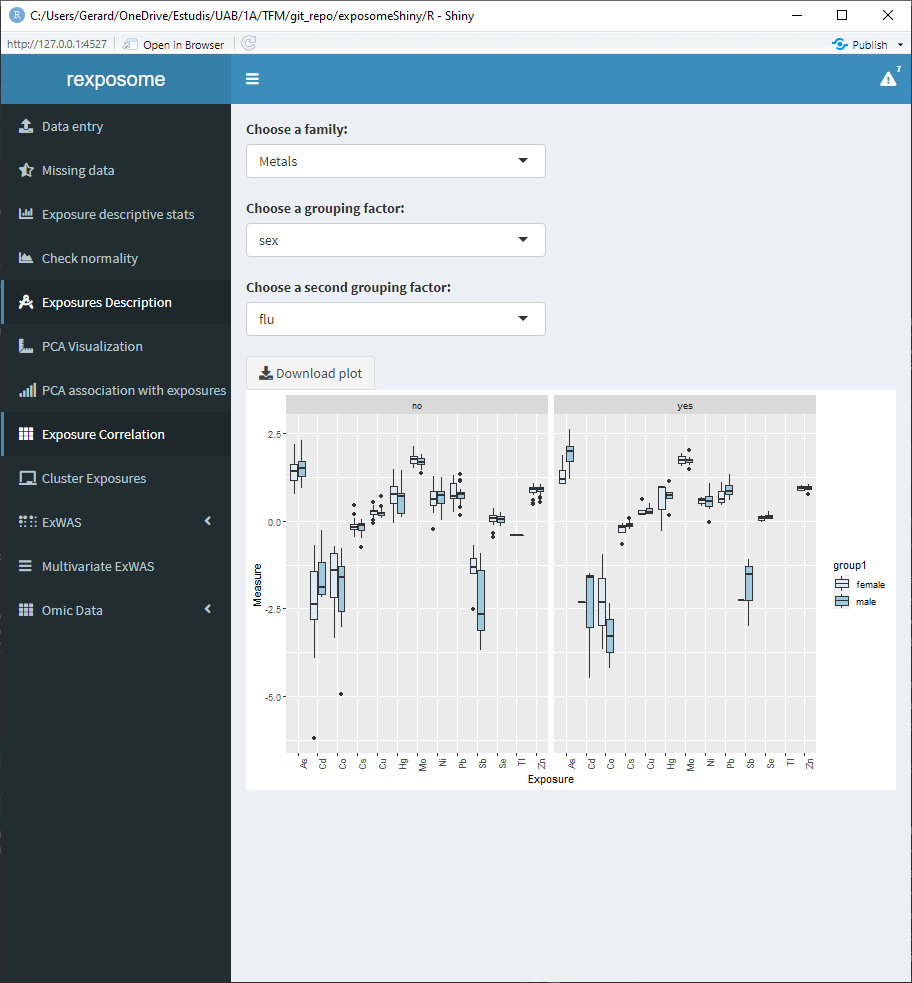
\includegraphics{images/analysis4_2_2.png}

\hypertarget{pca-analysis}{%
\subsection{PCA Analysis}\label{pca-analysis}}

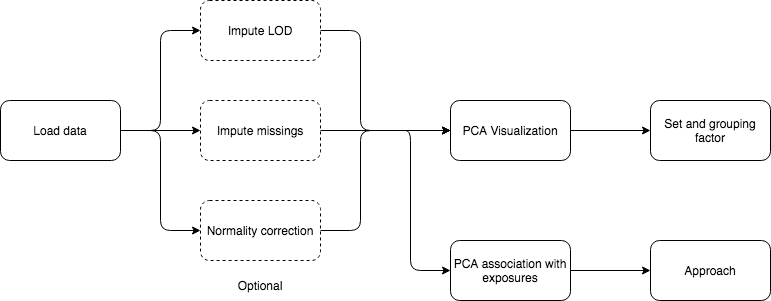
\includegraphics{images/analysis5_1.png}

On the `PCA visualization' tab, the results of a PCA analysis on the exposome data is displayed.

There are some input fields to modify the plot:

\begin{itemize}
\tightlist
\item
  Set: Select `all' to see an array of four plots with different PCA related information. There is also the option of selecting `samples' and `exposures' to only display those two plots on a bigger scale.
\item
  Grouping factor: To group the `samples' set using a qualitative phenotype.
\item
  Principal components: By default the first and second principal components are used for the plots. They can be changed using those inputs, which affect all the plots.
\end{itemize}

\hypertarget{set-all}{%
\subsubsection{Set: `all'}\label{set-all}}

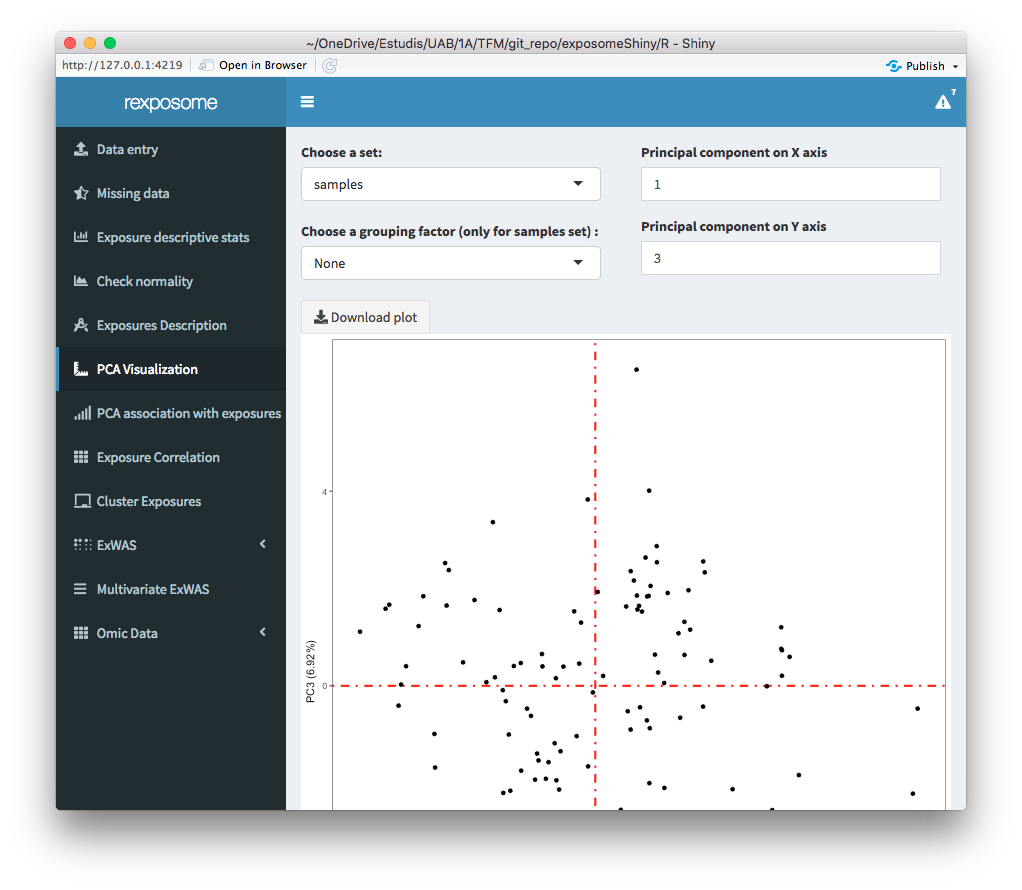
\includegraphics{images/analysis5_2.png}

\hypertarget{set-samples-grouped-by-sex}{%
\subsubsection{Set: `samples' grouped by sex}\label{set-samples-grouped-by-sex}}

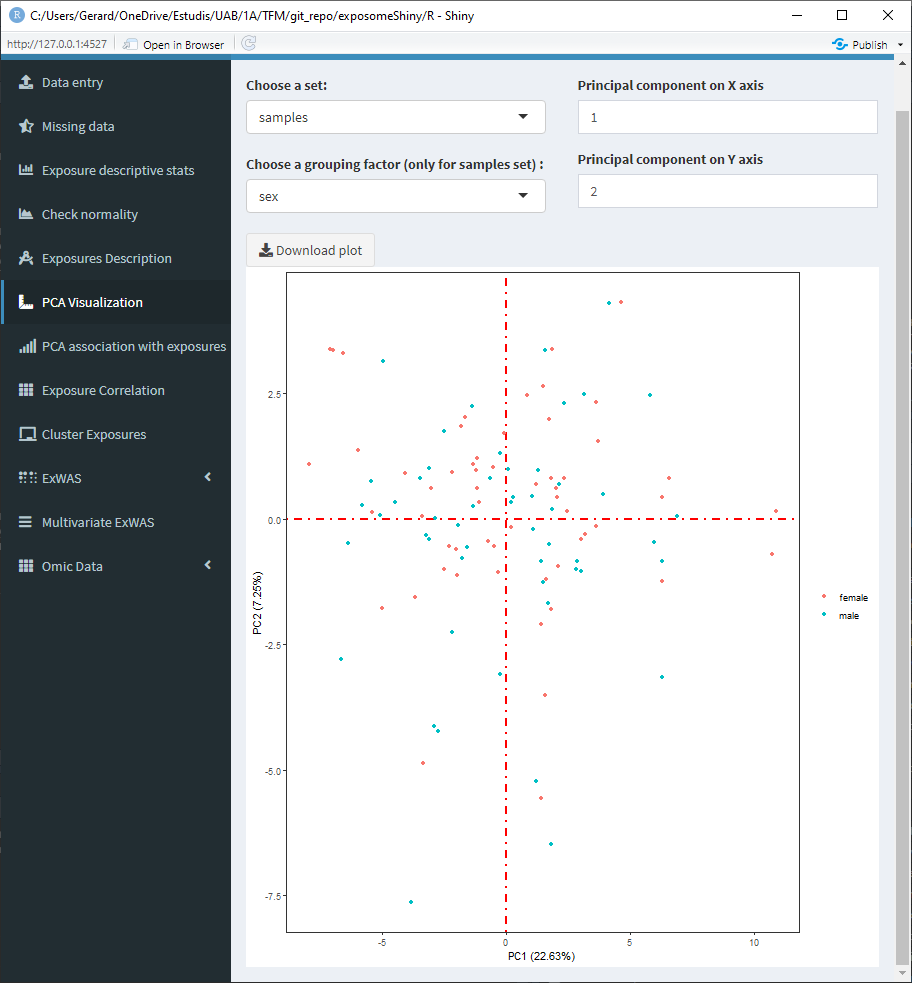
\includegraphics{images/analysis5_2_1.png}

\hypertarget{set-exposures}{%
\subsubsection{Set: `exposures'}\label{set-exposures}}

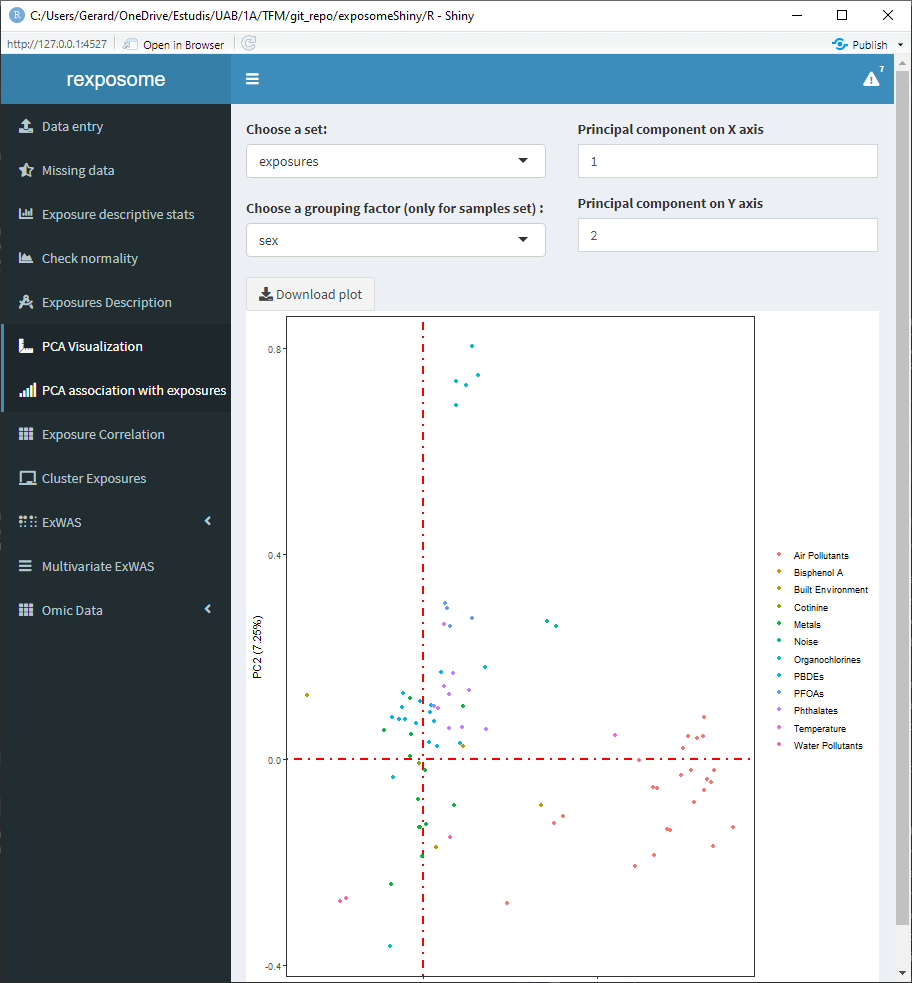
\includegraphics{images/analysis5_2_2.png}

Moreover, there is an additional PCA visualization tab named `PCA association with exposures'. On this tab there are two heatmap plots available.

\begin{itemize}
\tightlist
\item
  Association of the exposures to the principal components
\end{itemize}

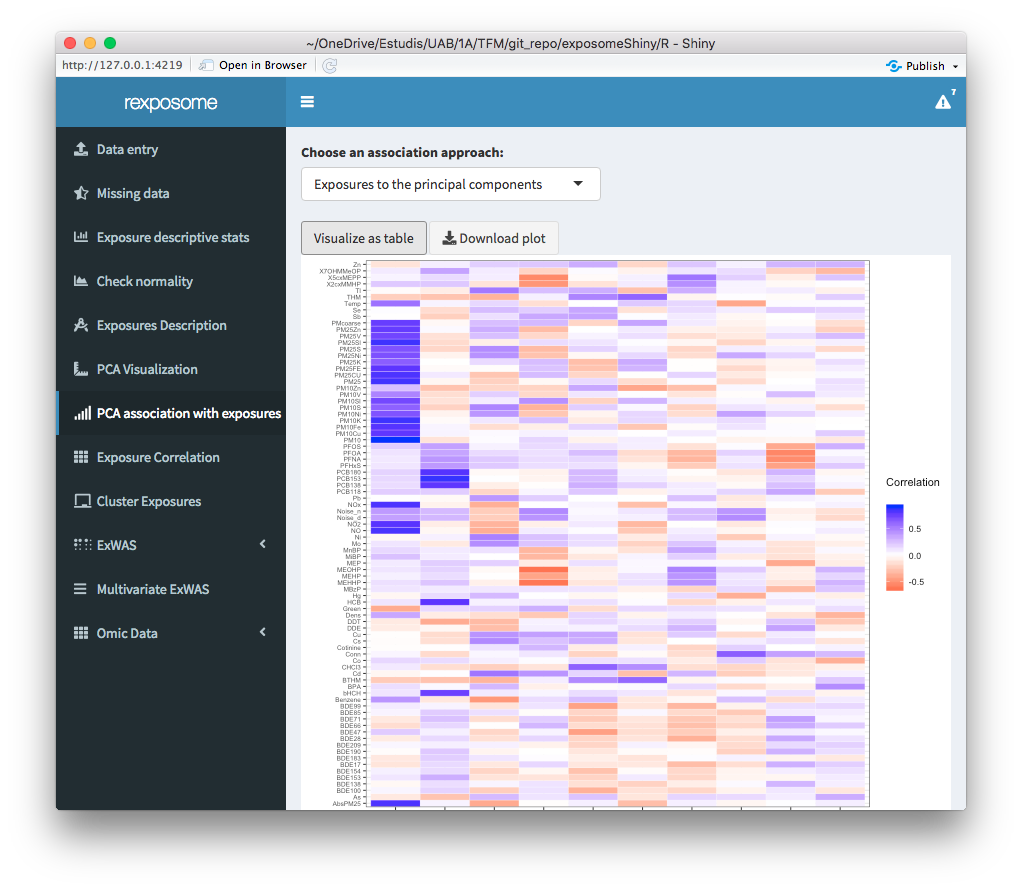
\includegraphics{images/analysis5_3.png}

\begin{itemize}
\tightlist
\item
  Association of the phenotypes to the principal components
\end{itemize}

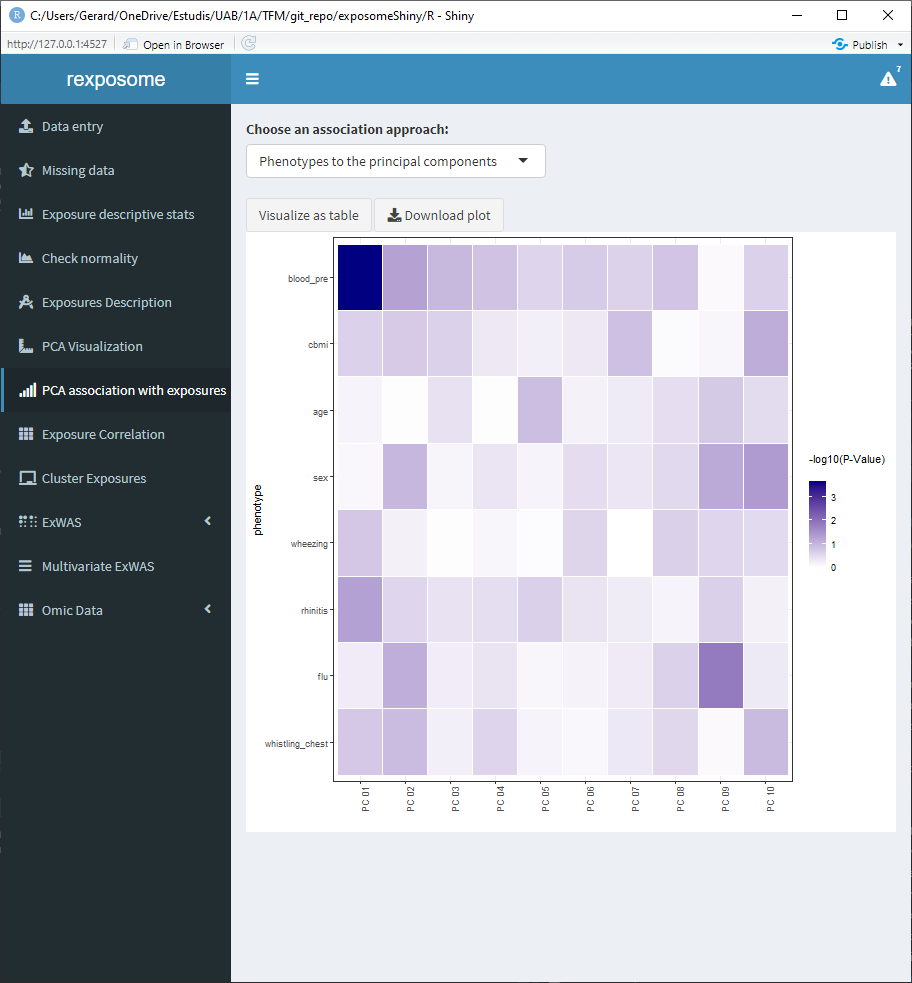
\includegraphics{images/analysis5_3_1.png}

The values of this heatmaps can be visualized as tables by clicking on `Visualize as table' and be downloaded as \texttt{*.csv}.

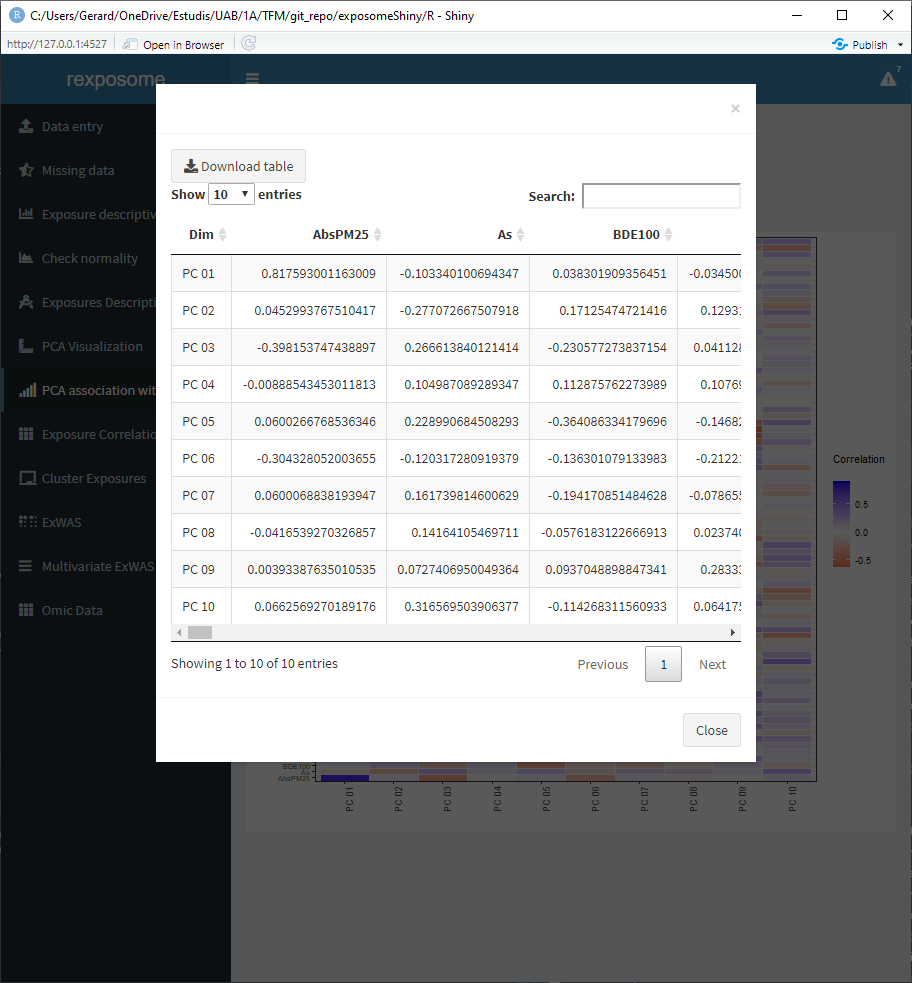
\includegraphics{images/analysis5_3_2.png}

\hypertarget{correlation-of-exposures}{%
\subsection{Correlation of exposures}\label{correlation-of-exposures}}

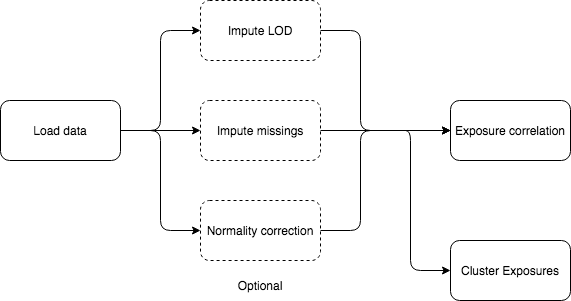
\includegraphics{images/analysis6_1.png}

Displaying the correlation of the exposures can help to visualize intra and inter family relations between the exposures, for that reason there are two different visualization options, the circos and the matrix.

The correlation is computed using Pearson method for numerical-to-numerical correlation, Cramer's V for categorical-to-categorical correlation and linear models for categorical-to-numerical.

\hypertarget{matrix-plot}{%
\subsubsection{Matrix plot}\label{matrix-plot}}

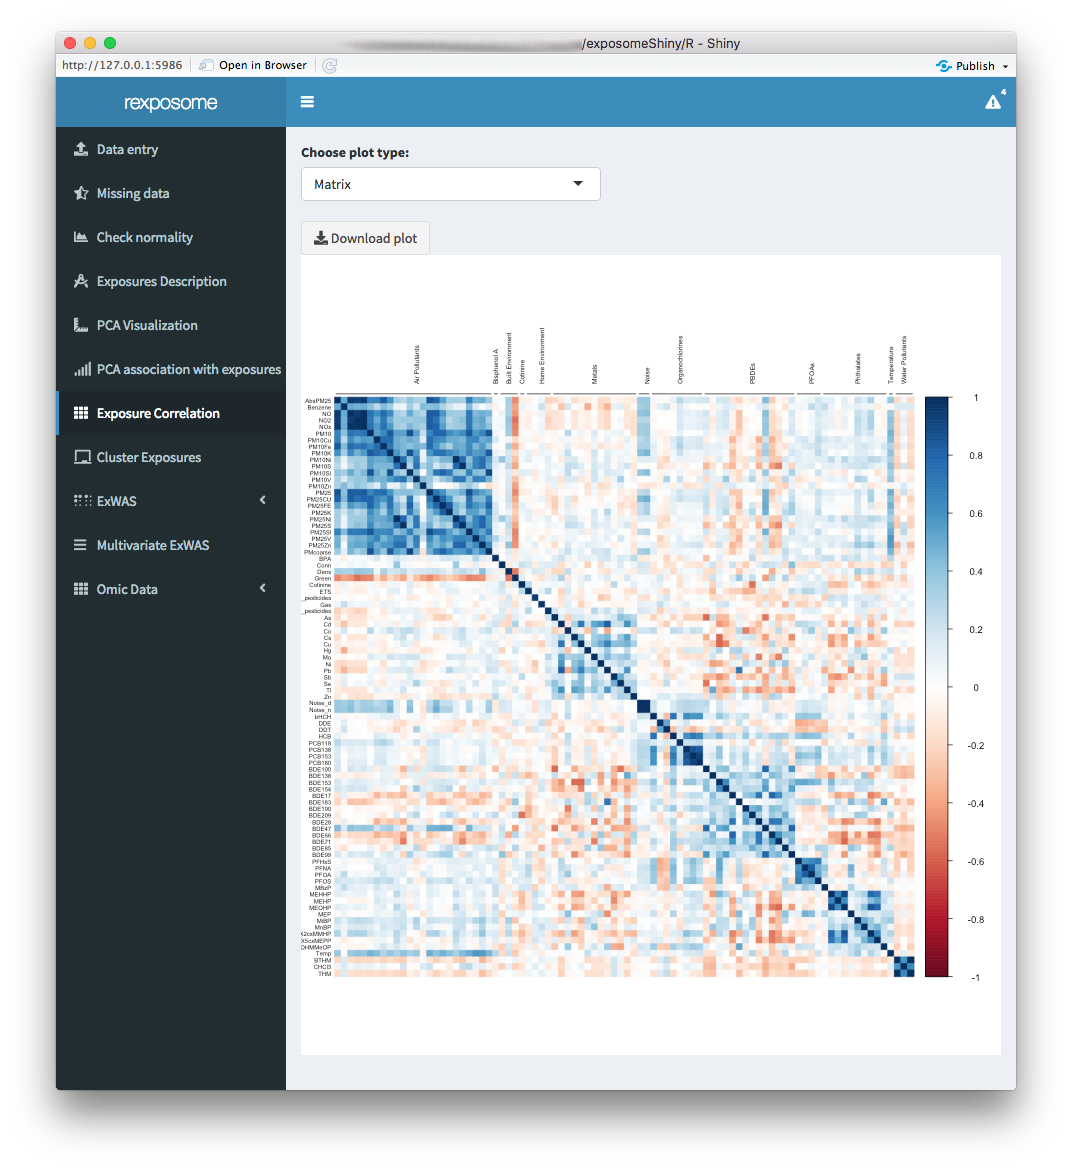
\includegraphics{images/analysis6_2.png}

\hypertarget{circos-plot}{%
\subsubsection{Circos plot}\label{circos-plot}}

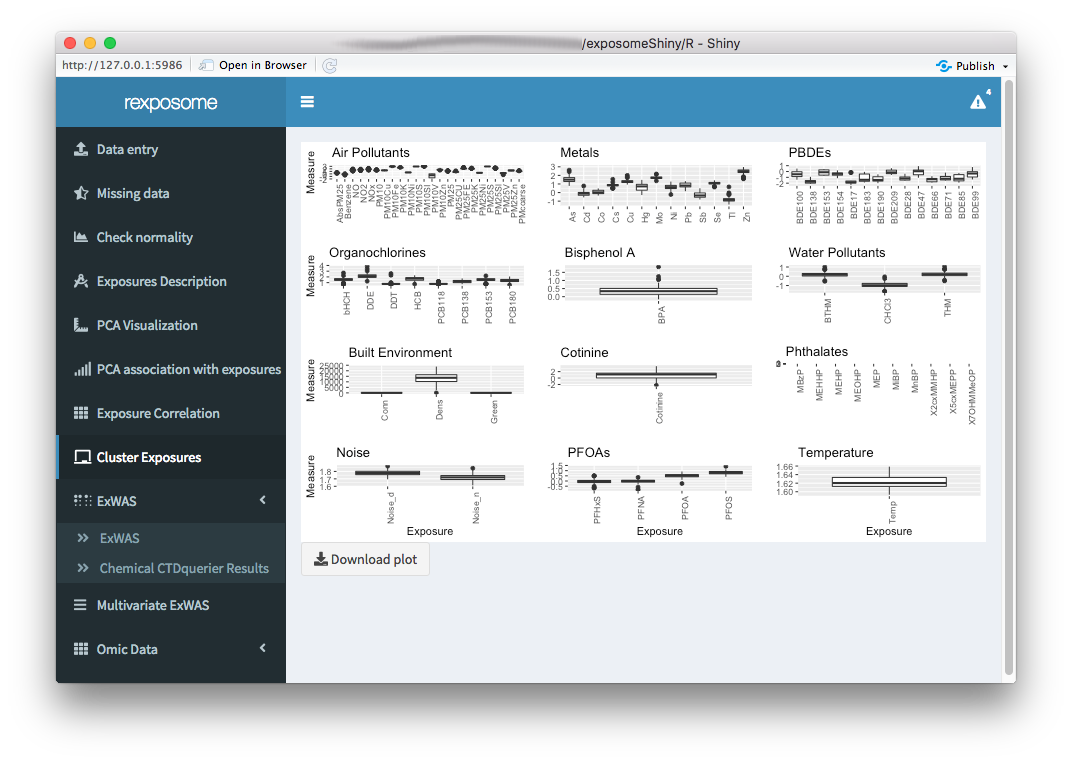
\includegraphics{images/analysis6_3.png}

\hypertarget{clusterization-of-exposures}{%
\subsection{Clusterization of exposures}\label{clusterization-of-exposures}}

The clusterization of exposures uses a hierarchical clustering algorithm to classify the individuals profiles of exposures in k groups, where k can be selected by the user. The plot shows the profile for each group of individuals.

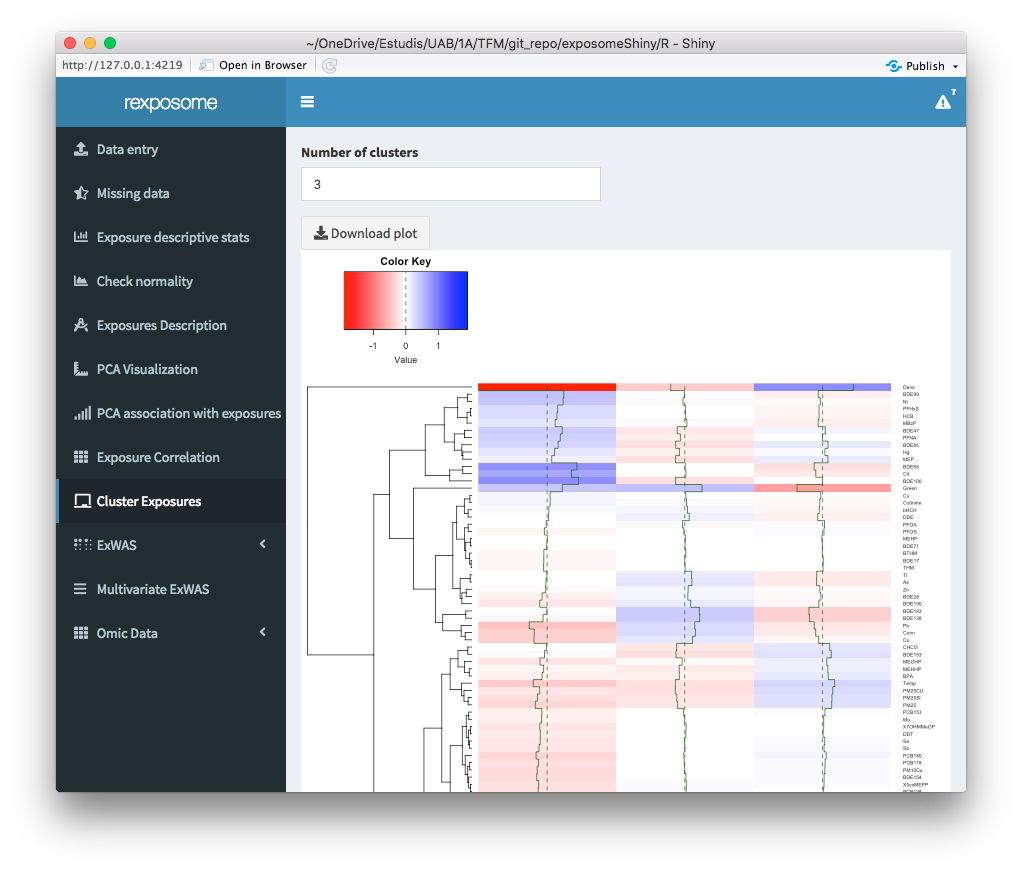
\includegraphics{images/analysis6_4.png}

\hypertarget{exwas}{%
\subsection{ExWAS}\label{exwas}}

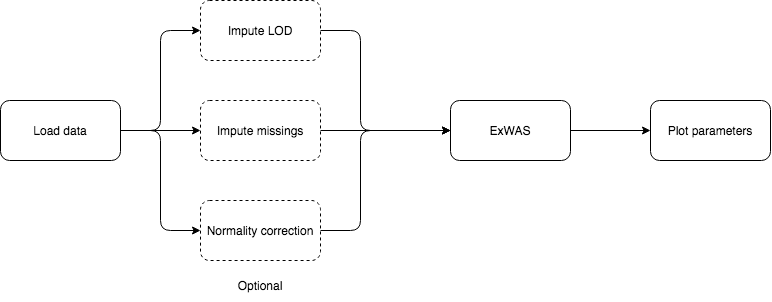
\includegraphics{images/analysis7_1.png}

There are two ExWAS methods implemented, the regular and the stratified. The difference is that the stratified performs multiple ExWAS subsetting the data with a quantitative phenotype (example: ExWAS with male data and ExWAS with female data).

To perfom an ExWAS enter the required fields:

\begin{itemize}
\tightlist
\item
  Outcome variable: Output phenotype
\item
  Covariable(s): Adjusting phenotype(s)
\item
  Output family: Family of the outcome variable (Gaussian/Binomial/Poisson)
\item
  Type of plot: Manhattan / Effects
\end{itemize}

\hypertarget{regular-exwas.-outcome-flu-covariable-sex-family-binomial}{%
\subsubsection{Regular ExWAS. Outcome: flu, Covariable: Sex, Family: Binomial}\label{regular-exwas.-outcome-flu-covariable-sex-family-binomial}}

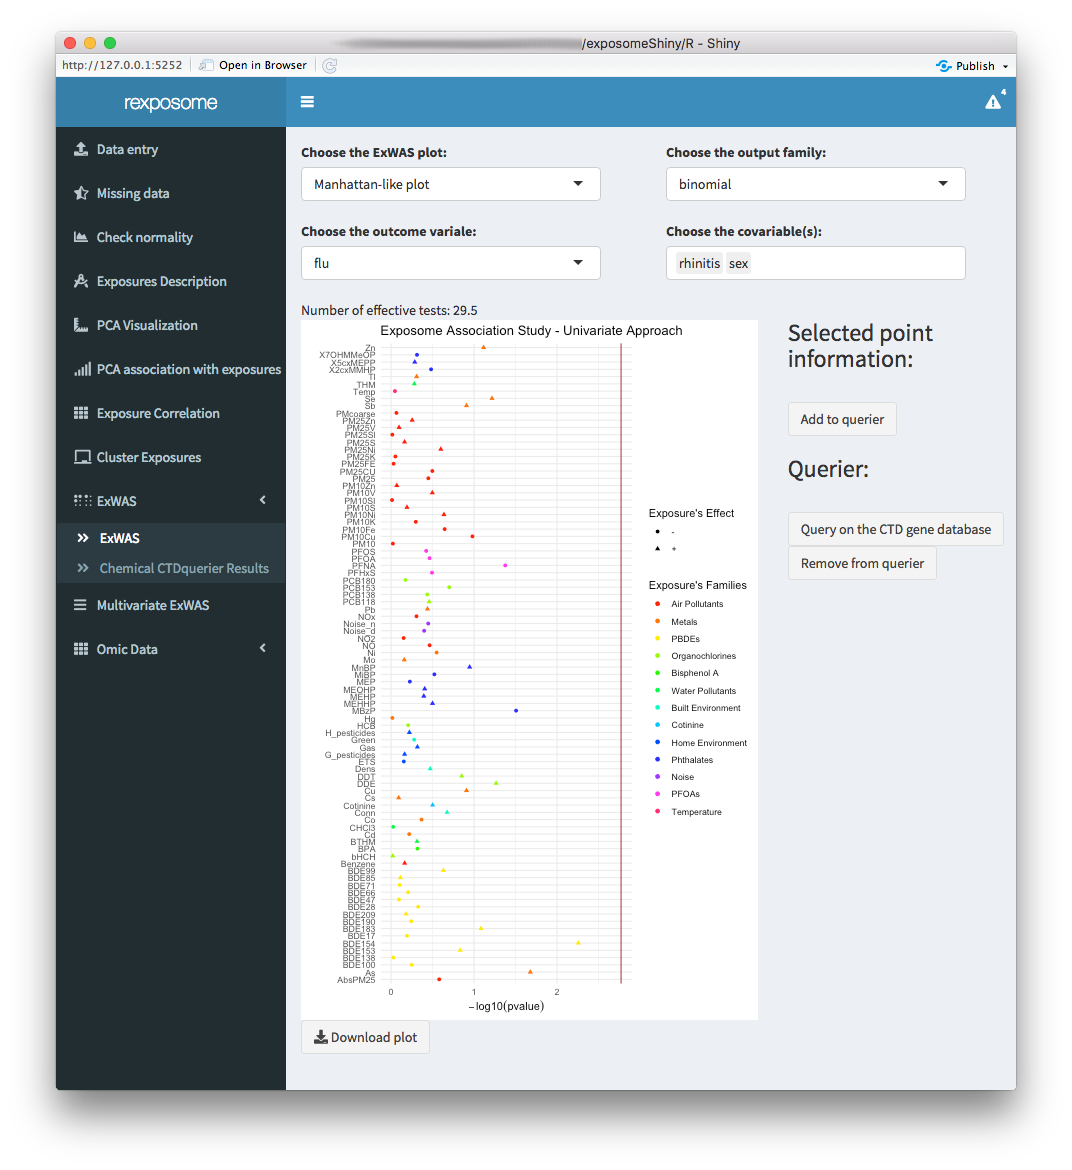
\includegraphics{images/analysis7_2.png}

\hypertarget{stratified-exwas.-outcome-flu-cobariable-none-family-binomial-stratifying-variable-sex}{%
\subsubsection{Stratified ExWAS. Outcome: flu, Cobariable: None, Family: Binomial, Stratifying variable: Sex}\label{stratified-exwas.-outcome-flu-cobariable-none-family-binomial-stratifying-variable-sex}}

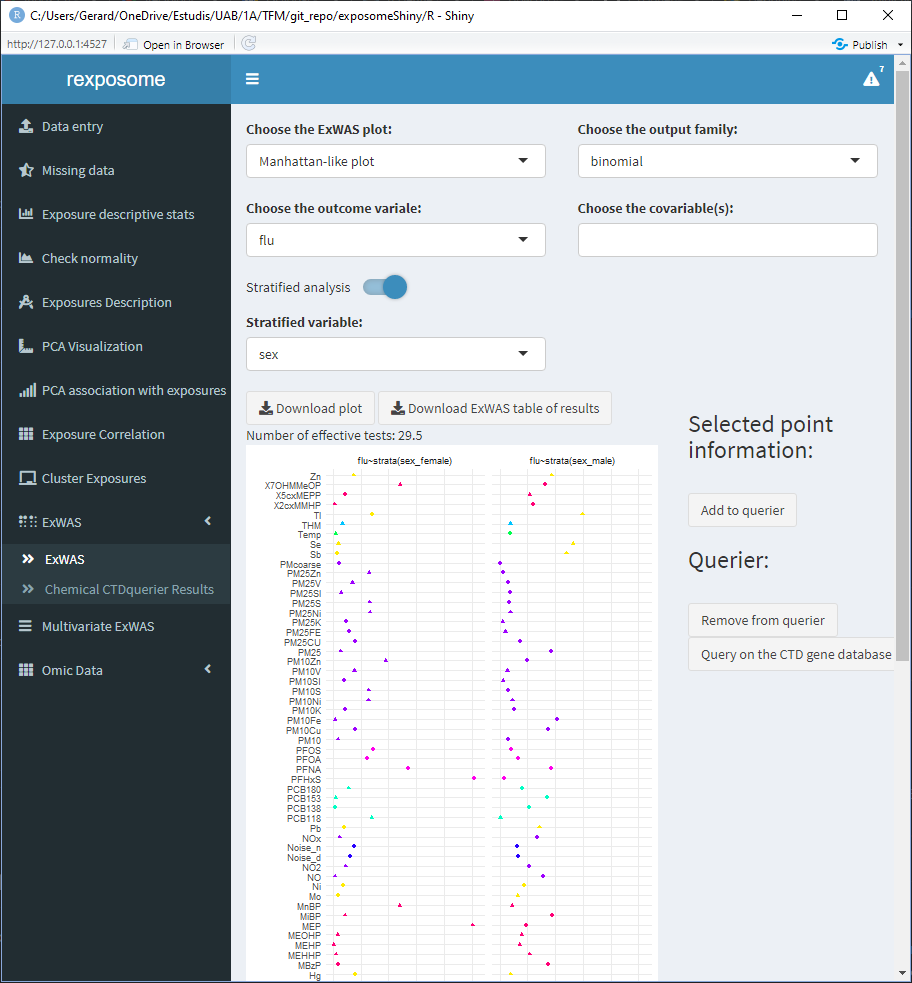
\includegraphics{images/analysis7_2_1.png}

The plots and results table can be downloaded. The results table contains the exposure names, association pvalue and effect (with CI 95\% for the effect). For the stratified ExWAS, the results table is actually a \texttt{*.zip} file with a file for each subset.

\hypertarget{exwas---ctdquerier}{%
\subsection{ExWAS - CTDquerier}\label{exwas---ctdquerier}}

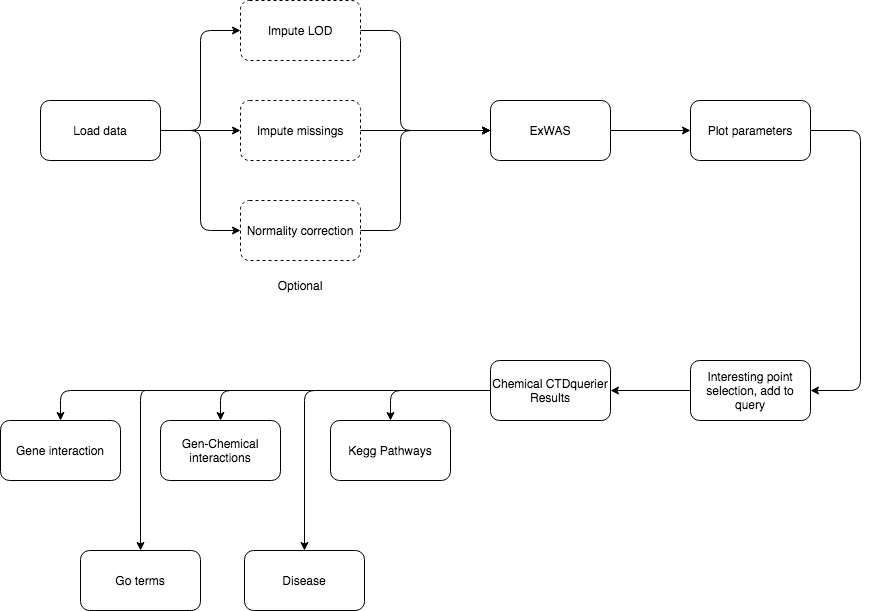
\includegraphics{images/analysis7_3.png}

The ExWAS analysis can reveal high association between health outcomes and exposures. To obtain further information (from the CTD database) on exposures of interest:

\begin{enumerate}
\def\labelenumi{\arabic{enumi}.}
\tightlist
\item
  Perform the ExWAS
\item
  Click on the exposure of interest on the plot
\item
  A table with information about the selected exposure will appear on the right
\end{enumerate}

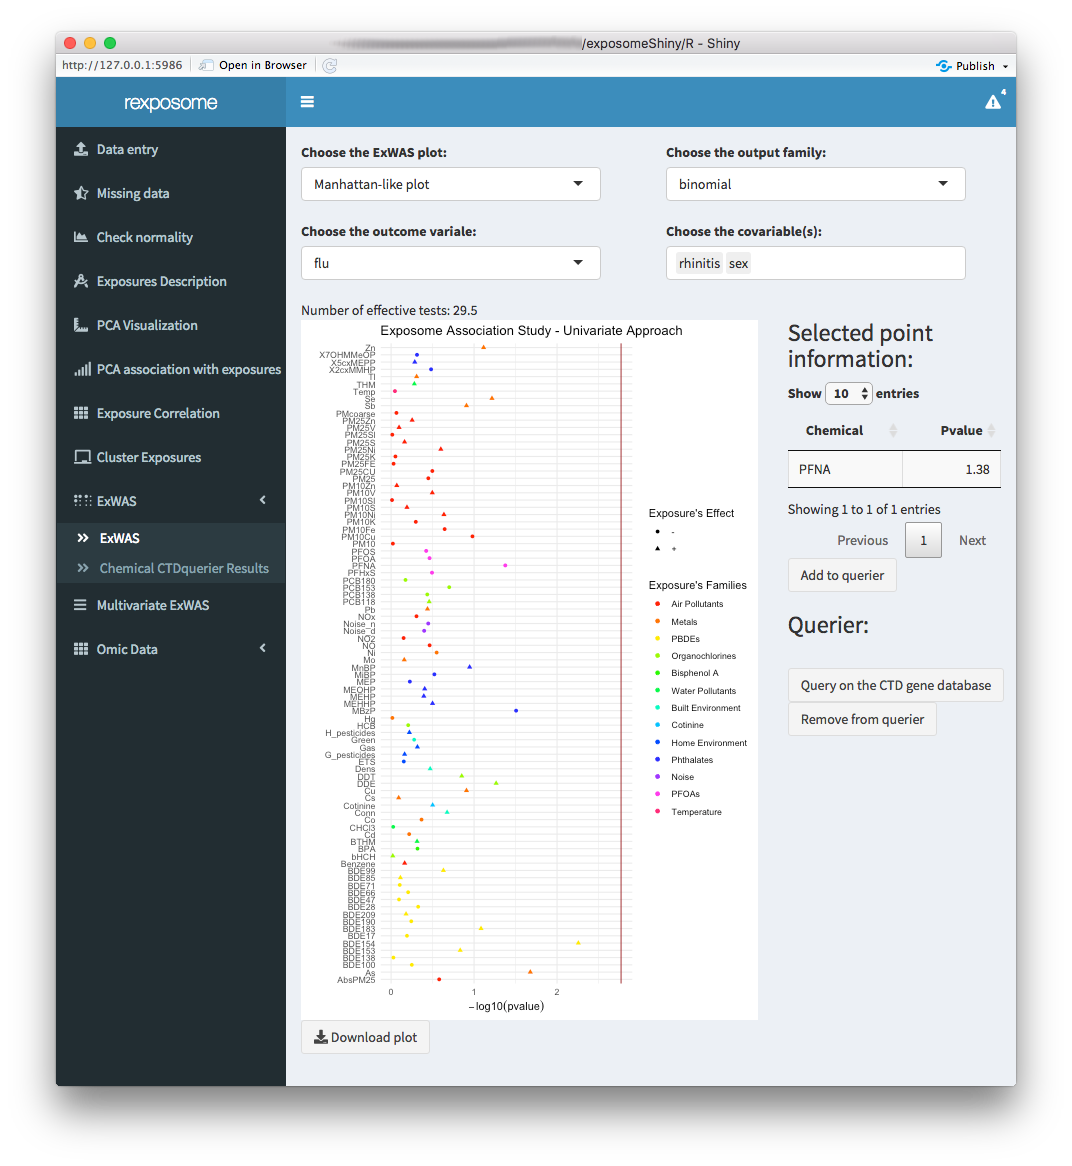
\includegraphics{images/analysis7_4.png}

\begin{enumerate}
\def\labelenumi{\arabic{enumi}.}
\setcounter{enumi}{3}
\tightlist
\item
  If the exposure shown on the right table is of interest, click on `Add to querier'
\end{enumerate}

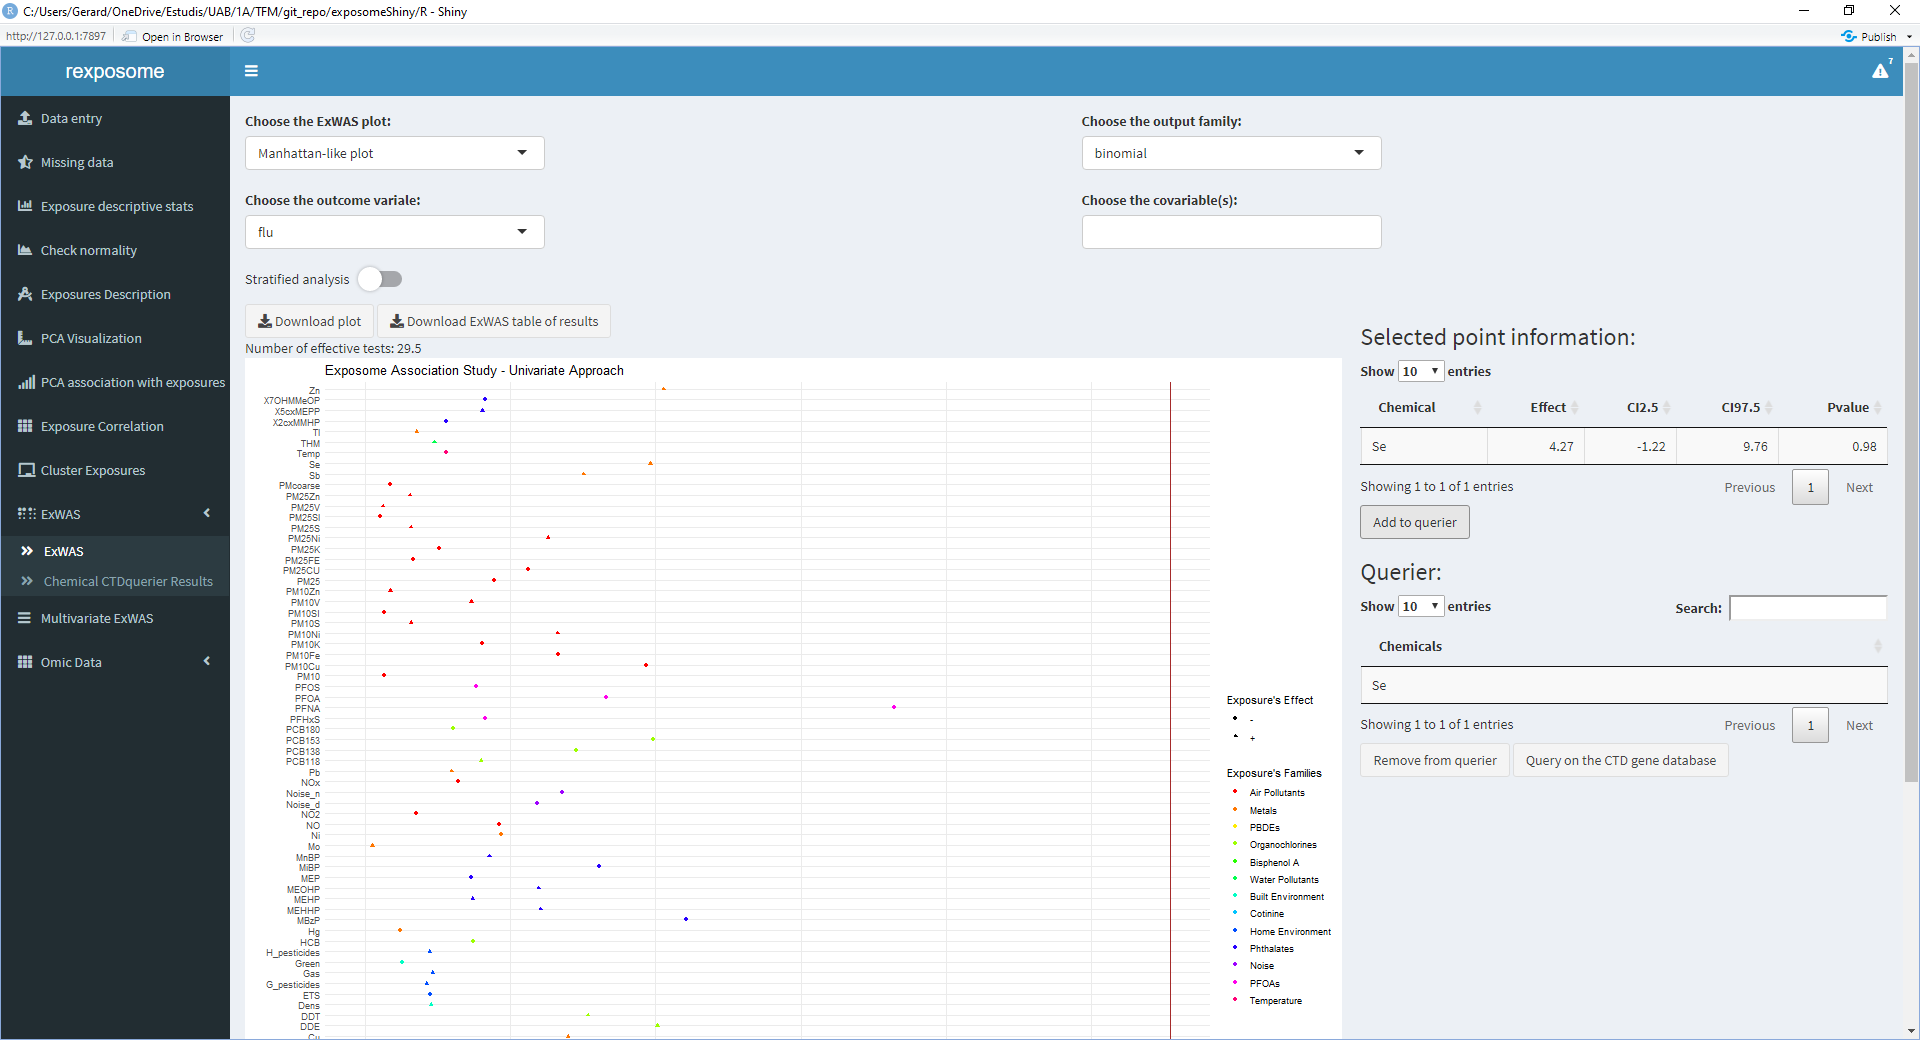
\includegraphics{images/analysis7_4_1.png}

\begin{enumerate}
\def\labelenumi{\arabic{enumi}.}
\setcounter{enumi}{4}
\tightlist
\item
  Repeat 2/3/4 for all the exposures of interest
\end{enumerate}

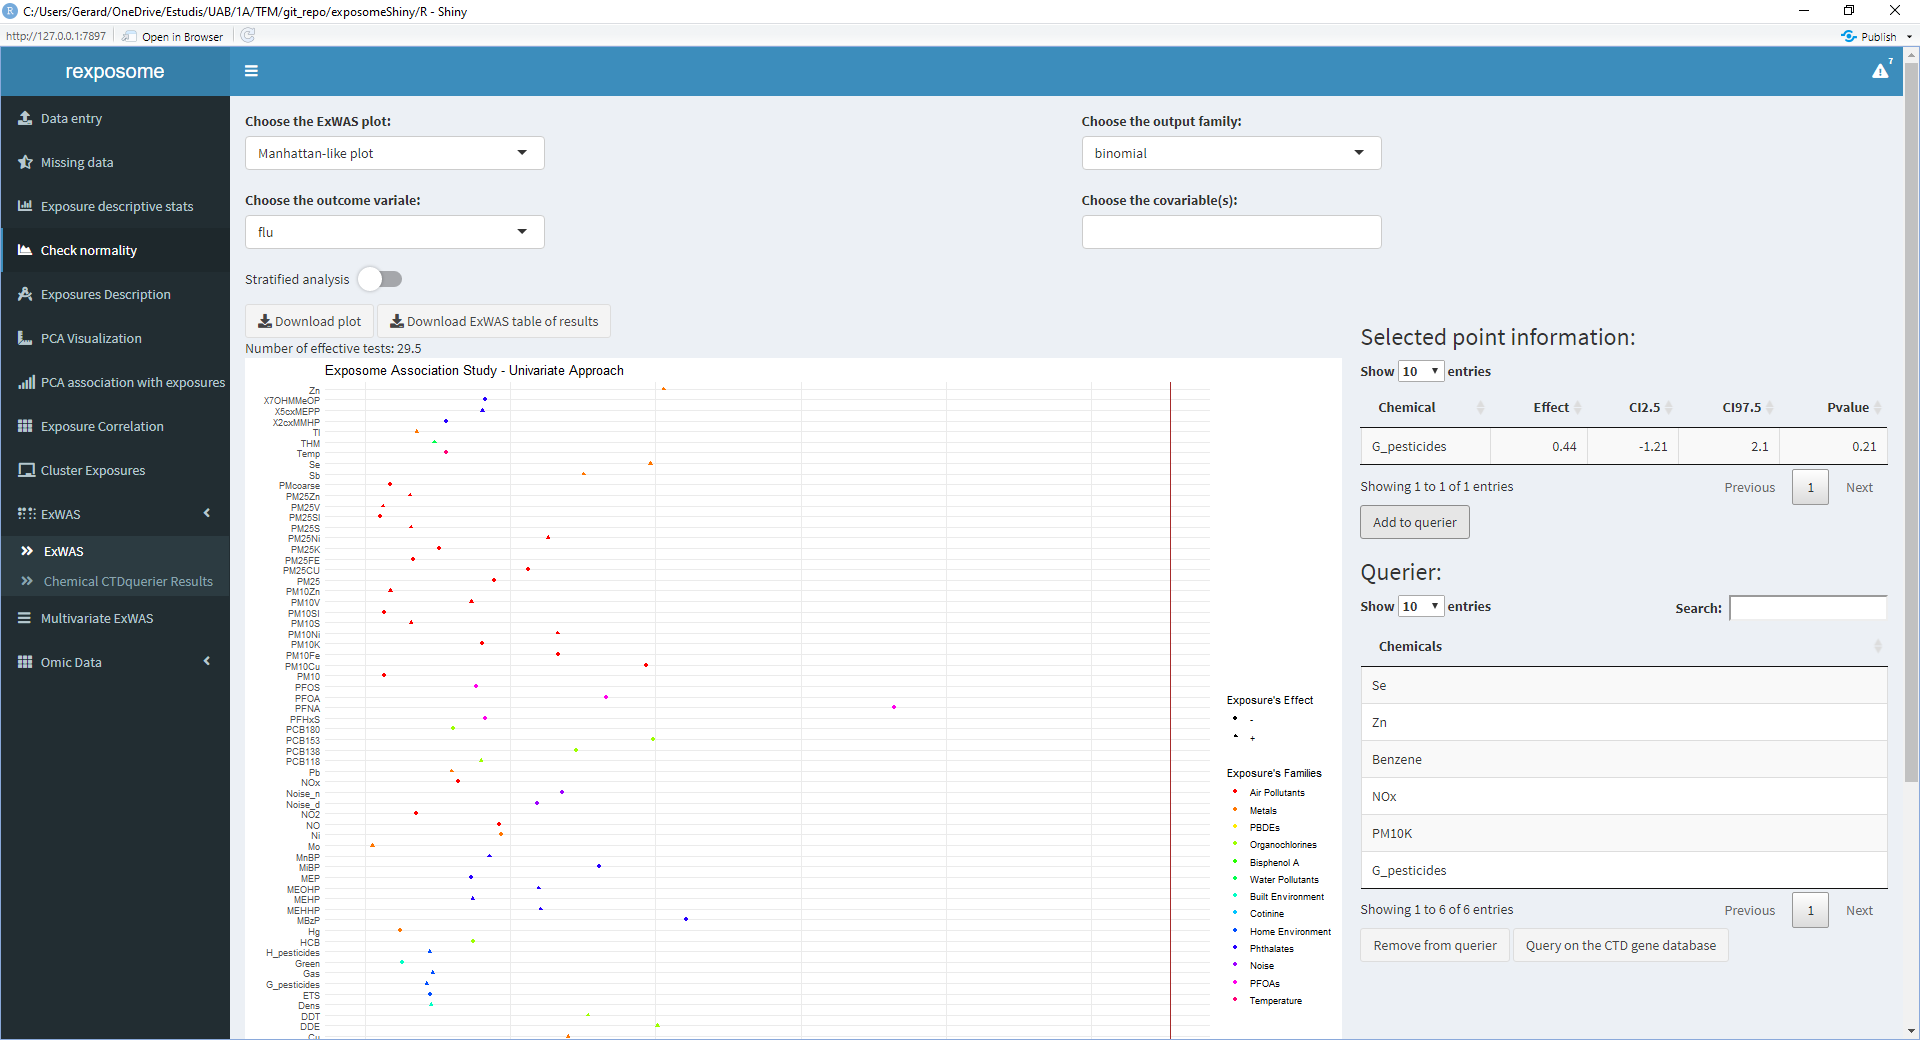
\includegraphics{images/analysis7_4_2.png}

\begin{enumerate}
\def\labelenumi{\arabic{enumi}.}
\setcounter{enumi}{5}
\tightlist
\item
  Once all the exposures of interest are on the `Querier' table, click `Query on the CTD gene database'
\end{enumerate}

The results of this query can be visualized on the `Chemical CTDquerier Results'. There are five visualization options:

\hypertarget{gene---chemical-interactions}{%
\subsubsection{Gene - chemical interactions}\label{gene---chemical-interactions}}

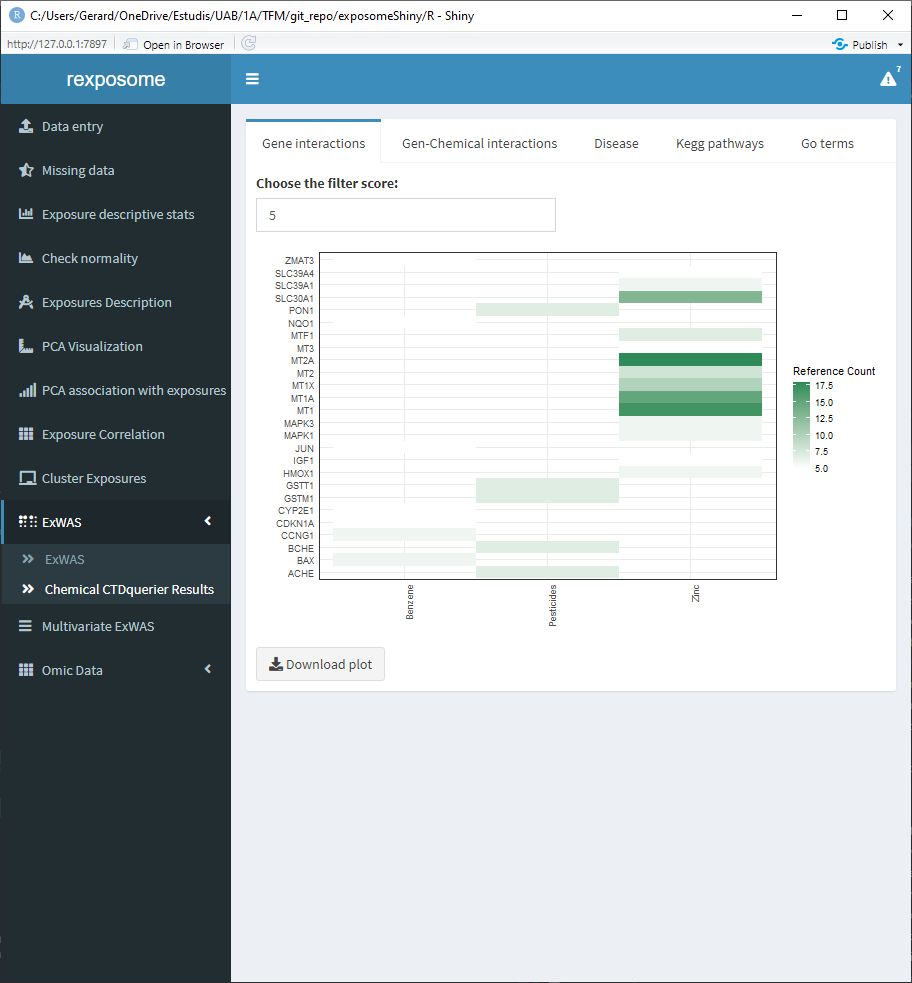
\includegraphics{images/analysis7_4_3.png}
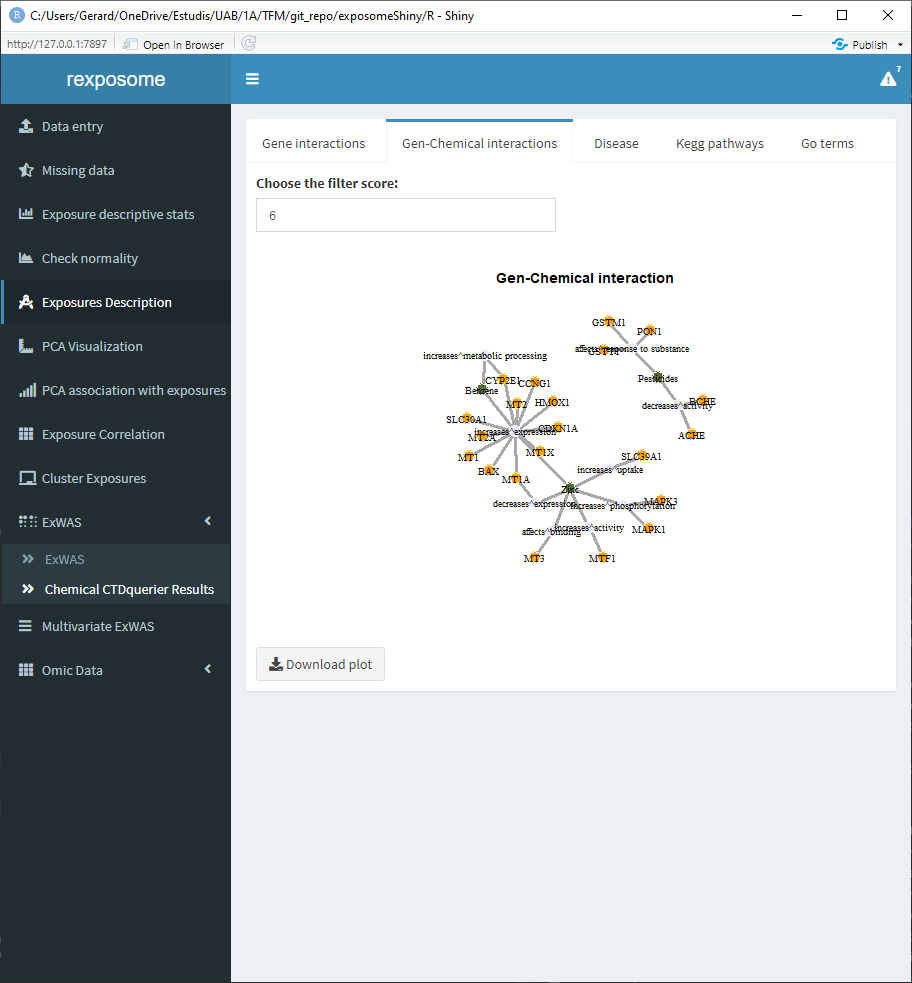
\includegraphics{images/analysis7_4_4.png}

\hypertarget{disease-relation}{%
\subsubsection{Disease relation}\label{disease-relation}}

\includegraphics{images/analysis7_4_5.png}

\hypertarget{kegg-pathways}{%
\subsubsection{Kegg pathways}\label{kegg-pathways}}

\includegraphics{images/analysis7_4_6.png}

\hypertarget{go-terms}{%
\subsubsection{Go terms}\label{go-terms}}

\includegraphics{images/analysis7_4_7.png}

\hypertarget{variable-selection-exwas}{%
\subsection{Variable selection ExWAS}\label{variable-selection-exwas}}

Variable selection ExWAS applies elastic net (LASSO regression) to the exposures given a health outcome of interest. The resulting heat map is coloured with the coefficient of each exposure in relation to the health outcome, so the ones in white are not associated. The two columns of the heat map correspond to the minimum lambda (\texttt{Min}) and to the lambda which gives the most regularized model such that error is within one standard error of the minimum (\texttt{1SE}).

\includegraphics{images/analysis8_1.png}

To perform a variable selection ExWAS study, check the Variable selection ExWAS tab and select the desired output parameter, click on run model to generate the plot.

This analysis requires data without missings, so if there are missings MICE imputation is applied beforehand. After the model is fitted, the imputed dataset will be removed.

\includegraphics{images/analysis8_2.png} \includegraphics{images/analysis8_3.png}

The table of results and plot can be downloaded.

\hypertarget{exposome-omic-analysis}{%
\section{Exposome-Omic analysis}\label{exposome-omic-analysis}}

The aim of this analysis is to perform an association test between the gene expression levels and the exposures. The datasets used in this section are \texttt{exposures.csv}, \texttt{description.csv}, \texttt{phenotypes.csv} and \texttt{gene\_exp.Rdata} which are available \href{https://github.com/isglobal-brge/exposomeShiny/tree/master/data}{here}.

It's important noting that (by default) the maximum size of the omics data is 30 MB, if the omics file to be analyzed is bigger, change the line number 2 of the \texttt{server.R} file.

\begin{Shaded}
\begin{Highlighting}[]
  \CommentTok{\# the "30" refers to 30MB, change as needed}
\FunctionTok{options}\NormalTok{(}\AttributeTok{shiny.maxRequestSize=}\DecValTok{30}\SpecialCharTok{*}\DecValTok{1024}\SpecialCharTok{\^{}}\DecValTok{2}\NormalTok{)}
\end{Highlighting}
\end{Shaded}

\hypertarget{association-analysis}{%
\subsection{Association analysis}\label{association-analysis}}

\includegraphics{images/analysis9_1.png}

First, make sure that the exposome dataset is loaded. Then, proceed to loading the omics data, which should be providad as a \texttt{*.RData}.

\includegraphics{images/analysis9_2.png}

This type of analysis is usually very computationally intensive, so it's useful to be able to limit the scope. The exposome data can be subsetted by families for that reason. If all the families are desired don't input any and proceed to click the ``Subset and add''.

\includegraphics{images/analysis9_3.png}

Select the variables for the association analysis (linear models) and if SVA (surrogate variable analysis) is wanted on the ``Association model'' subtab.

\includegraphics{images/analysis9_4.png}

Once complete, there are various tabs to visualize the results.

The ``Results table'' shows the gene, log of the fold change, p-value and adjusted p-value.

\includegraphics{images/analysis9_5.png}

The ``Significant hits'' shows the exposure, hits and lambda.

\includegraphics{images/analysis9_6.png}

The QQ Plot shows a QQ plot (expected vs.~observed -lo10(p-value)) for the selected exposure.

\includegraphics{images/analysis9_7.png}

The Volcan plot shows a volcano plot (log2(fold change) vs -log10(p-value)). For this plot there are two input cells to adjust the horizontal and verital limit lines to filter out the results.

\includegraphics{images/analysis9_8.png}

\hypertarget{ctd-querier}{%
\subsection{CTD querier}\label{ctd-querier}}

\includegraphics{images/analysis10_1.png}

The association analysis of exposome data and omic data may point some genes of interest. Information about these genes can be queried on the CTD database.

To do so:

\begin{enumerate}
\def\labelenumi{\arabic{enumi}.}
\tightlist
\item
  Perform association analysis
\item
  Go to the volcano plot visualization
\item
  Select one point. This will update the `Selected point information' table at the bottom
\end{enumerate}

\includegraphics{images/analysis10_2.png}

Sometimes multiple points may be very close, so this table will show information about them

\includegraphics{images/analysis10_2_1.png}

\begin{enumerate}
\def\labelenumi{\arabic{enumi}.}
\setcounter{enumi}{3}
\tightlist
\item
  Select the point of interest from the `Selected point information' table and click on `Add to querier'. This will the search of the gene related to the selected SNP. Sometimes the search may not yield a resulting gene.
\end{enumerate}

\includegraphics{images/analysis10_2_2.png}

\begin{enumerate}
\def\labelenumi{\arabic{enumi}.}
\setcounter{enumi}{4}
\tightlist
\item
  Repeat 3/4 for all the points of interest
\end{enumerate}

\includegraphics{images/analysis10_2_3.png}

When all the genes of interest are on the querier, move to the `CTDquerier' tab. On it, the genes to be queried can be visualized before performing the query. Once the query is performed, the results can be visualized on the different tabs.

\includegraphics{images/analysis10_3.png}

There are six tabs showing different results interpretations. First there's the ``Lost \& found'' tab which a plot to see the amount of genes found on the CTD database and the ones that were not found , there's also two lists stating the names of them.

\includegraphics{images/analysis10_4.png}

The diseases tab shows a table of all the associated diseases found on the CTD database.

\includegraphics{images/analysis10_5.png}

The curated diseases tab shows the table of associated diseases but only shows the ones with direct evidence.

\includegraphics{images/analysis10_6.png}

The association tab shows information about all the direct evidence associated diseases. Select the disease of interest to see the score and reference count of it.

\includegraphics{images/analysis10_7.png}

The inference score tab shows the inference score for each gene for a selected disease, the filter parameters puts out the genes with an inference score lower than the selected filter.

\includegraphics{images/analysis10_8.png}

The association matrix tab shows a matrix of genes vs.~chemicals with a heatmap representing the existing papers (references) providing evidence about the association between chemicals and genes.

\includegraphics{images/analysis10_9.png}

\hypertarget{enrichment-analysis}{%
\subsection{Enrichment analysis}\label{enrichment-analysis}}

\includegraphics{images/analysis11.png}

To perform an enrichment analysis, select the genes of interest by following the same procedure as with the CTDquerier.

After selecting them, go to the ``Enrichment analysis'' tab, on it there is a selector to choose between GO and KEGG databases and a threshold selector for the cutoff pvalue of the enrichment analysis.

\includegraphics{images/analysis11_1.png}

When the enrichment analysis is performed, there are multiple visualization tabs for the results, the first one is a table with the plain results, which can be downloaded.

\includegraphics{images/analysis11_2.png}

The following four tabs correspond to different visualization options for the results. All of them can be downloaded.

\includegraphics{images/analysis11_3.png}
\includegraphics{images/analysis11_4.png}
\includegraphics{images/analysis11_5.png}
\includegraphics{images/analysis11_6.png}

\hypertarget{exposome-omic-integration-e.g.-crossomics}{%
\section{Exposome-Omic integration (e.g.~crossomics)}\label{exposome-omic-integration-e.g.-crossomics}}

The datasets used in this section are \texttt{exposures\_2.csv}, \texttt{description\_2.csv}, \texttt{phenotypes\_2.csv}, \texttt{brge\_gexp.rda} and \texttt{brge\_prot.rda} which are available \href{https://github.com/isglobal-brge/exposomeShiny/tree/master/data}{here}.

\includegraphics{images/analysis12.png}

The relation between exposures and omic-features can be studied from another perspective, different from the association analyses. The integration analysis can be done, using multi canonical correlation analysis, multiple co-inertia analysis or partial least squares (this method only is supported with one omics dataset). The first method is implemented in R package \texttt{PMA} (CRAN) and the second in \texttt{omicade4} R package (Bioconductor). The PLS uses the \texttt{mixOmics} R package (Bioconductor).

Before conducting an integration model, an exposome dataset has to be loaded into the Shiny application.

For the MCIA and MCCA options, the exposome dataset can't contain missings, so it needs to be imputed beforehand. For the PLS there can be missings. Different visualizations are provided for each method, as the used R packages provide different visualization tools, all three methods generate different plots. The Rdata object that contains the results can be downloaded to be explorated by the user on a separate R session.

The differences between association and crossomics are that the first method test association between two complete data-sets, by removing the samples having missing values in any of the involved data-sets, and the second try to find latent relationships between two or more sets.

The initial page of the integration is the following.

\includegraphics{images/analysis12_1.png}

The user has a field to select a omics file and a `Type of file' field. This text field is to input whether the selected data is expression/proteome/\ldots{} this field will be used for informative purposes when displaying the results.

If more than one omics dataset is going to be used on the integration, click on `More data' to get additional input fields, remember that only MCIA and MCCA accept more than one omics dataset.

\includegraphics{images/analysis12_2.png}

Once the data entry is completed, click on `Load data and perform integration'. Go to the results page to see the plots of the integration.

The following screenshots are the results of an integration analysis using the exposome dataset (\texttt{exposures\_2.csv}, \texttt{description\_2.csv}, \texttt{phenotypes\_2.csv}) with the missings imputed (using the `Missing data' tab of the Shiny) expression omics (\texttt{brge\_gexp.rda}) and proteome omics (\texttt{brge\_prot.rda}). All this mentioned datasets can be found \href{https://github.com/isglobal-brge/exposomeShiny/tree/master/data}{here}.

\hypertarget{integration-using-mcia}{%
\subsection{Integration using MCIA}\label{integration-using-mcia}}

\includegraphics{images/analysis12_3.png}

\hypertarget{integration-using-mcca-using-only-the-proteome-omics}{%
\subsection{Integration using MCCA (using only the proteome omics)}\label{integration-using-mcca-using-only-the-proteome-omics}}

\includegraphics{images/analysis12_4.png}

\hypertarget{integration-using-pls-using-only-the-proteome-omics}{%
\subsection{Integration using PLS (using only the proteome omics)}\label{integration-using-pls-using-only-the-proteome-omics}}

There are multiple visualization options for the PLS integration.

\hypertarget{the-exposures-space}{%
\subsubsection{The exposures space}\label{the-exposures-space}}

Can be grouped using the categorical phenotypes of the exposome data

\includegraphics{images/analysis12_5.png}

\hypertarget{the-variables-space}{%
\subsubsection{The variables space}\label{the-variables-space}}

\includegraphics{images/analysis12_6.png}

\hypertarget{a-correlation-heatmap}{%
\subsubsection{A correlation heatmap}\label{a-correlation-heatmap}}

Available for the first three principal components

\includegraphics{images/analysis12_7.png}

\hypertarget{loading-plots-coefficients-of-each-variable}{%
\subsubsection{Loading plots (coefficients of each variable)}\label{loading-plots-coefficients-of-each-variable}}

Available for the first three principal components

\includegraphics{images/analysis12_8.png}

All plots can be downloaded individually, also, the Rdata file that contains the results of the integration can be downloaded.

\hypertarget{general-application-functionalities}{%
\chapter{General application functionalities}\label{general-application-functionalities}}

This whole Shiny application serves the purpose to perform a various number of exposome and omic analysis with an input set of data. To perform this analysis some operations can performed on the inputed dataset prior to the analysis and so in order to follow track of what exactly has been done or what is loaded on the current session, there's implemented some sort of state tracker inside the Shiny application. In order to access it, press the icon on the top right of the application

\includegraphics{images/general1.png}

When clicking it a dropdown menu appears, inside there are seven different notifications:

\begin{itemize}
\tightlist
\item
  Exposome dataset: Turns to 100\% when an exposome dataset is loaded in the environment. Here's a graphical example.

  \includegraphics{images/general2.png}

  \includegraphics{images/general3.png}
\item
  LOD imputed: Turns to 100\% if the exposome dataset is LOD imputed.
\item
  Missing imputed: Turns to 100\% if the exposome dataset has the missings imputed.
\item
  Normality corrected: Turns to 100\% if the exposome dataset is normality corredted.
\item
  Omics dataset: Turns to 100\% when an omics dataset is loaded in the environment.
\item
  Subset: Turns to 100\% (and displays the subset family(ies)) when the exposome dataset is subseted.
\item
  Model: Turns to 100\% (and displays the association variable(s)) when a model is performed for an omics association analysis. Here's an example of a subset and model information.

  \includegraphics{images/general4.png}
\end{itemize}

\hypertarget{methods}{%
\chapter{Methods}\label{methods}}

\hypertarget{missing-data-imputation}{%
\section{Missing data imputation}\label{missing-data-imputation}}

LOD missings are discovered through a encoding provided by the user, there is no method implemented to separate missing values between missing at random at LOD, meaning that all NA values are considered missing at random.

\hypertarget{limit-of-detection-lod-missing}{%
\subsection{Limit of detection (LOD) missing}\label{limit-of-detection-lod-missing}}

LOD missings can be imputed using two methodologies:

\begin{itemize}
\tightlist
\item
  LOD value / sqrt(2) : Use a LOD value provided by the user (one value per exposures) divided by the square root of two. \citet{Richardson2003}
\item
  QRILC: a quantile regression approach for the imputation of left-censored missing data \citet{lod_impute}.
\end{itemize}

\hypertarget{missing-at-random}{%
\subsection{Missing at random}\label{missing-at-random}}

Multiple imputation chained equations (MICE) is used to impute missing at random data. The \emph{mice} package is used to do so. A brief explanation on the algorithm:

\begin{enumerate}
\def\labelenumi{\arabic{enumi}.}
\tightlist
\item
  Imputation of the variable (exposure) xn with the mean of all it's values.
\item
  Perform 1 for all the variables.
\item
  Set the mean imputed values from one variable back to missing.
\item
  Perform a regression model and fill those missings.
\item
  Repeat 3 and 4 for all the variables.
\item
  Repeat 3, 4 and 5 until the imputed values obtained are stabilized.
\end{enumerate}

\hypertarget{normality}{%
\section{Normality}\label{normality}}

\hypertarget{normality-testing}{%
\subsection{Normality testing}\label{normality-testing}}

To test the normality of a variable, a Shapiro-Wilks test is used. The Shapiro-Wilks test, tests the null hypothesis of a sample (variable of the dataset) is normally distributed, to perform the test it calculates the W statistic.

\(W = \frac{\left( \Sigma^{n}_{i=1} a_i x_{(i)} \right)^2}{\Sigma^{n}_{i=1} (x_i - \overline{x})^2}\)

To perform this test exposome uses the \emph{shapiro.test} function from the \emph{base} package of R.

\hypertarget{normalization}{%
\subsection{Normalization}\label{normalization}}

A user selected function can be applied to exposures (selected by the user) to normalize them. The available functions are: \emph{log}, \emph{sqrt} and \emph{\^{}1/3}.

\hypertarget{principal-component-analysis-pca}{%
\section{Principal component analysis (PCA)}\label{principal-component-analysis-pca}}

Rexposome contains two PCA methodologies

\begin{itemize}
\tightlist
\item
  Regular PCA \citet{Jolliffe2016} (only numerical exposures)
\item
  FAMD \citet{chavent2014multivariate} (numerical and categorical)
\end{itemize}

exposomeShiny uses regular PCA from the \emph{FactoMineR} package. A toggle to select between the two may be added in future releases.

\hypertarget{exposures-correlation}{%
\section{Exposures correlation}\label{exposures-correlation}}

The correlation method takes into account the nature of each pair of exposures: continuous vs.~continuous uses cor function from R \emph{base}, categorical vs.~categorical uses cramerV function from \emph{lsr} R package and categorical vs.~continuous exposures correlation is calculated as the square root of the adjusted r-square obtained from fitting a lineal model with the categorical exposures as dependent variable and the continuous exposure as independent variable.

\hypertarget{exposures-clustering}{%
\section{Exposures clustering}\label{exposures-clustering}}

Clustering analysis on samples can be performed to cluster individuals having similar exposure profiles. This is done using hierarchical clustering using the function \emph{hclust} from the \emph{stats} R package. The results this analysis yields are the exposure profiles of a selected number of groups.

\hypertarget{exposome-association-analysis}{%
\section{Exposome Association Analysis}\label{exposome-association-analysis}}

\hypertarget{single-association-analysis}{%
\subsection{Single Association Analysis}\label{single-association-analysis}}

Exposome-Wide Association Study (ExWAS) is equivalent to a Genome-Wide Association Study (GWAS) in genomics or to Epigenetic-Wide Association Study (EWAS) in epigenomics. The ExWAS was first described by Patel et al. \citet{patel2010environment} . ExWAS are based on generalized linear models using any formula describing the model that should be adjusted for (following standard formula options in R). That is, continuous or factor variables can be incorporated in the design, as well as interaction or splines using standard R functions and formulas. Multiple comparisons in the ExWAS analysis is addressed by computing the number of effective (Neff) tests as described by Li and Ju \citet{li2005adjusting} . The method estimates Neff by using the exposure correlation matrix that is corrected when it is not positive definite by using \emph{nearPD} R function. The significant threshold is computed as 1-(1-0.05)Meff. This threshold is added to the Manhattan plots. When using imputed data, analysis is done for each imputed set and P-Values are pooled to obtain a global association score.

\hypertarget{stratified-single-association-analysis}{%
\subsection{Stratified Single Association Analysis}\label{stratified-single-association-analysis}}

The stratified analysis option for the ExWAS corresponds to applying the same method as regular ExWAS to subsetted datasets. As example, a stratified analysis with the \texttt{sex} variable stratified corresponds to performing two ExWAS, one to the \texttt{male} and one for the \texttt{female} group.

\hypertarget{variable-selection-exwas-1}{%
\subsection{Variable selection ExWAS}\label{variable-selection-exwas-1}}

There are some authors that proposed to perform association analysis in a multivariate fashion, just to take into account the correlation across exposures \citet{agier2016systematic} . A Lasso regression is implemented using Elastic-Net regularized generalized linear models implemented in \emph{glmnet} R package.

\hypertarget{exposome-omic-association-analysis}{%
\section{Exposome-Omic Association Analysis}\label{exposome-omic-association-analysis}}

Perform association analyses between exposures and omic data bt fitting linear models as described in the \emph{limma} R package \citet{ritchie2015limma} . The pipeline implemented in association allows performing surrogate variable analysis in order to correct for unwanted variability. This adjustment is provided by \emph{SVA} R package \citet{sva} .

\hypertarget{integration-analysis}{%
\section{Integration analysis}\label{integration-analysis}}

There are three different methodologies to perform the integration analysis:

\begin{itemize}
\tightlist
\item
  Multiset canonical correlation analysis (MCCA). Implemented using the \texttt{MultiCCA} function of \texttt{PMA} R package \citet{witten2020package} .
\item
  Multiple co-inertia analysis (MCIA). Implemented using the \texttt{mcia} function of \texttt{omicade4} R package \citet{mcia} , \citet{min2020sparse} .
\item
  Partial least squares (PLS). Implemented using the \texttt{plsr} function of \texttt{pls} R package \citet{mevik2015introduction} .
\end{itemize}

\hypertarget{enrichment-analysis-1}{%
\section{Enrichment analysis}\label{enrichment-analysis-1}}

Functional profiles of selected genes are obtained using the Bioconductor package \texttt{clusterProfiler} \citet{clusterprofiler} . The available enrichment databases are GO and KEGG.

\hypertarget{references}{%
\chapter{References}\label{references}}

\hypertarget{refs}{}
\begin{CSLReferences}{0}{0}
\end{CSLReferences}

  \bibliography{book.bib,packages.bib}

\end{document}
